% $Id: sttt.tex,v 1.65 2004/11/26 10:49:42 erikpoll Exp $
%
\begin{filecontents}{leer.eps}
%!PS-Adobe-2.0 EPSF-2.0
%%CreationDate: Mon Jul 13 16:51:17 1992
%%DocumentFonts: (atend)
%%Pages: 0 1
%%BoundingBox: 72 31 601 342
%%EndComments

gsave
72 31 moveto
72 342 lineto
601 342 lineto
601 31 lineto
72 31 lineto
showpage
grestore
%%Trailer
%%DocumentFonts: Helvetica
\end{filecontents}
%

\documentclass[sttt]{svjour}
% Remove option referee for final version

\usepackage{url}
\usepackage{ifpdf}
\usepackage{verbatim}
\usepackage{floatflt}
\usepackage{graphicx}

% Choose one of the two definitions, for draft or public versions.
\newcommand{\TODO}[1]{\textbf{[[#1]]}}
% \newcommand{\TODO}[1]{\relax}

% Names of tools (commands), so we change have a consistent and
% uniform style for them.
\newcommand{\CMD}[1]{\textit{#1}}
\newcommand{\JML}{\CMD{jml}}
\newcommand{\JMLC}{\CMD{jmlc}}
\newcommand{\JMLUNIT}{\CMD{jmlunit}}
\newcommand{\JMLSPEC}{\CMD{jmlspec}}
\newcommand{\JMLDOC}{\CMD{jmldoc}}
\newcommand{\JAVADOC}{\CMD{javadoc}}
\newcommand{\MJDOC}{\CMD{mjdoc}}
\newcommand{\JMLRAC}{\CMD{jmlrac}}
\newcommand{\ESCJAVA}{\CMD{ESC/Java}}
\newcommand{\ESCJAVATWO}{\CMD{ESC/Java2}}
\newcommand{\ESCJAVAS}{\CMD{ESC/Java(2)}}
\newcommand{\JACK}{\CMD{JACK}}
\newcommand{\Daikon}{\CMD{Daikon}}
\newcommand{\Houdini}{\CMD{Houdini}}
\newcommand{\CHASE}{\CMD{ChAsE}}
\newcommand{\LOOP}{\CMD{LOOP}}
\newcommand{\Krakatoa}{\CMD{Krakatoa}}
\newcommand{\Jive}{\CMD{Jive}}
\newcommand{\KeY}{\CMD{KeY}}

\hyphenation{JUnit}
\hyphenation{JML-an-no-tat-ed}
\hyphenation{as-sign-able}

\begin{document}

\title{An overview of JML tools and applications}
\author{Lilian Burdy\inst{1} \and
        Yoonsik Cheon\inst{2} \and
        David R. Cok\inst{3} \and
        Michael D. Ernst\inst{4} \and
        Joseph R. Kiniry\inst{5} \and
        Gary T. Leavens\inst{6}\thanks{Supported in part by US NSF grants CCR-0097907 and CCR-0113181} \and
        K. Rustan M. Leino \inst{7} \and
        Erik Poll\inst{5}
       }
 \institute{INRIA, Sophia-Antipolis, France
           \and
           Dept. of Computer Science,
           University of Texas at El Paso,
           El Paso, Texas, USA
           \and
           Eastman Kodak Company, R\&D Laboratories, Rochester, New York, USA
           \and
           Computer Science \& Artificial Intelligence Lab, MIT,
           Cambridge, Massachusetts, USA
           \and
           Dept. of Computer Science,
           University of Nijmegen,
           Nijmegen, the Netherlands
           \and
           Dept. of Computer Science,
           Iowa State University,
           Ames, Iowa, USA
           \and 
           Microsoft Research,
           Redmond, Washington, USA }



\date{Received: date / Revised version: date}
% The correct dates will be entered by Springer

\authorrunning{Burdy et al.}

\maketitle

\begin{abstract}
  The Java Modeling Language (JML) can be used to specify the detailed
  design of Java classes and interfaces by adding annotations to Java
  source files.  The aim of JML is to provide a specification language
  that is easy to use for Java programmers and that is supported by a
  wide range of tools for specification type-checking, runtime
  debugging, static analysis, and verification.
  
  This paper gives an overview of the main ideas behind JML, 
  details about JML's wide range of tools, and a glimpse into
  existing applications of JML\@.
\end{abstract}

%=====================================================================
\section{Introduction}

JML~\cite{Leavens-Baker-Ruby99b,Leavens-Baker-Ruby03}, the
Java Modeling Language, is useful for specifying detailed
designs of Java classes and interfaces.  JML is a behavioral interface
specification language for Java; that is, it specifies both the behavior
and the syntactic interface of Java code.  The syntactic interface of
a Java class or interface consists of its method signatures,
the names and types of its fields, etc.
This is what is commonly meant by an application programming
interface (API).
The behavior of such an API can be precisely documented in JML annotations;
these describe the intended way that programmers should
use the API\@.  In terms of behavior, JML can detail, for example, the
preconditions and postconditions for methods as well as class
invariants, in the \emph{Design by Contract} style~\cite{Meyer97}.
\begin{floatingfigure}{2.5cm} % {0.50\columnwidth}
%% [[[Need the pdf version to be committed for pdflatex]]]
\centering
\ifpdf
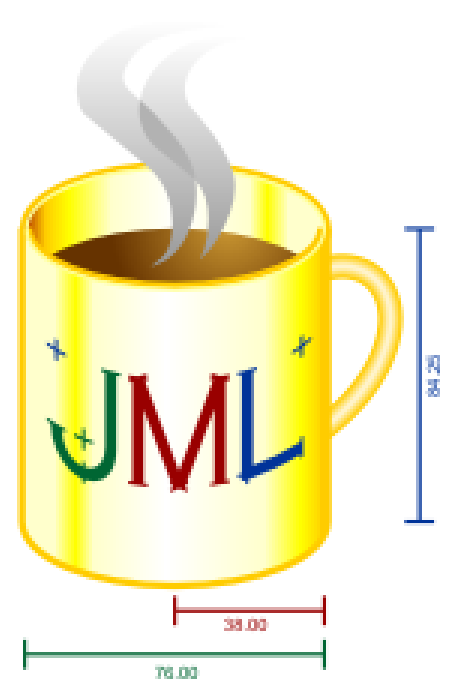
\includegraphics[width=2.5cm]{jmllogo}
\else
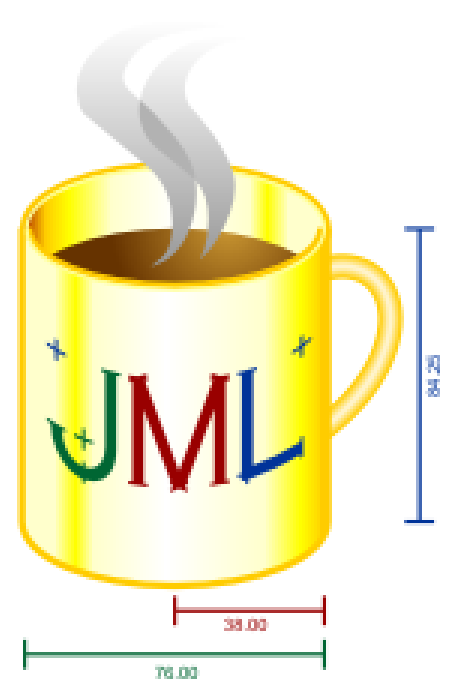
\includegraphics[width=2.5cm]{jmllogo.eps}
\fi
%
\end{floatingfigure}

An important goal for the design of JML is that it should be easily
understandable by Java programmers. This is achieved by staying as
close as possible to Java syntax and semantics.  Another important
design goal is that JML \emph{not} impose any particular design methodology
on users; instead, JML should be able to document Java programs
designed in any manner.

The work on JML was started by Gary Leavens and his colleagues and
students at Iowa State University. It has since grown into a cooperative,
open effort.  Several groups worldwide are now building tools that
support the JML notation and are involved with the ongoing design of
JML\@.  
For an up-to-date list, see the JML website, \url{www.jmlspecs.org}.
The open, cooperative nature of the JML effort is important
both for tool developers and users, and we welcome participation by
others.  For potential users, the fact that there are several tools
supporting the same notation is clearly an advantage.  For tool
developers, using a common syntax and semantics can make it much
easier to get users interested. After all, one of the biggest hurdles
to using a new specification-centric tool is often the lack of
familiarity with the associated specification language.
%% [[[Comment from referee 2 about the above:]]]
% I certainly do not subscribe to the authors view
% that the biggest hurdle to formal methods adoption is the overhead of
% having to learn another language - in my experience this is simply false.
% Any tool with sufficient return on investment will be used.

\medskip

The next section introduces the JML notation.  Sections~\ref{tools}
through \ref{toolsEnd} then discuss the tools currently available for
JML in more detail.  Section~\ref{applications} discusses the
applications of JML in the domain of Java Card, the Java dialect for
programming smartcards.  Section~\ref{related} discusses some related
languages and tools,
% Section~\ref{future-work} lays out future work,
and Section~\ref{conclusions} concludes.

%=====================================================================
\section{The JML Notation}
\label{notation}

JML blends Eiffel's \emph{Design by Contract} approach~\cite{Meyer97} with
the Larch tradition \cite{Guttag-Horning93,Cheon-Leavens94,Leavens96b}
(both of which share features and ideas with VDM \cite{Jones90}).\footnote{
JML also has takes some features from the refinement calculus
\cite{Morgan94}, which we do not discuss in this paper.
}
Because JML supports quantifiers such as
\verb_\forall_ and \verb_\exists_, and because JML allows model
(i.e., specification-only) fields and methods, specifications can
easily be made more precise and complete than is typical for Eiffel software.
However, following Eiffel's use of its expression syntax in assertions,
JML uses Java's expression syntax in assertions;
this makes JML's notation easier for programmers to learn than notations
based on a language-independent specification language,
such as the Larch Shared
Language~\cite{Leavens-Baker-Ruby03,Leavens-etal03b} or
OCL~\cite{WarmerKleppe99}.

%% Note that I have used the newly specified constructor to illustrate
%% a point about ESC/Java below, so beware if you try to save space by
%% deleting it. -- Gary
%% I added a checkPin method to illustrate some points about the runtime assertion checker -- Gary

% position at the center; argument is the width of the text.
\newenvironment{centertext}[1]{%
   \begin{center}\begin{minipage}{#1}}
  {\end{minipage}\end{center}}

\begin{figure*}
%
\begin{centertext}{5.25in}
\verbatiminput{Purse.java}
\end{centertext}
%
\caption{\label{example}Example JML specification}
\end{figure*}

Figure~\ref{example} gives an example of a JML specification that
illustrates its main features.  JML assertions are written as special
annotation comments in Java code,
either after \verb_//@_ or between \verb_/*@ ... @*/_,
so that they are ignored by Java compilers but can be used
by tools that support JML\@.  Within annotation comments, JML extends the
Java syntax with several keywords---in the example in
Figure~\ref{example}, the JML keywords \texttt{invariant},
\texttt{requires}, \texttt{assignable}, \texttt{ensures}, and
\texttt{signals} are used.  It also extends Java's expression syntax
with several operators---in the example \verb_\forall_, \verb_\old_, and
\verb_\result_ are used; these begin with a backslash so they do not
clash with existing Java identifiers.

The central ingredients of a JML specification are preconditions
(given in \texttt{requires} clauses), postconditions (given in
\texttt{ensures} clauses), and invariants.  These are 
all expressed as boolean expressions in JML's extension to Java's
expression syntax.

In addition to \emph{normal} postconditions, the language also supports
\emph{exceptional} postconditions, specified using \texttt{signals} clauses.
These can be used to specify what must be true when a method throws an
exception.  For example, the \texttt{signals} clause in
Figure~\ref{example}'s \texttt{debit} method specifies that 
\texttt{debit} may
throw a \texttt{PurseException} and that the balance will not change
in that case (as specified by the use of the \verb+\old+ keyword).

The \texttt{assignable} clause for the method \texttt{debit} specifies a
frame condition, namely that \texttt{debit} will assign only to the
\texttt{balance} field.  Although not a traditional part of Design by
Contract languages like Eiffel, such frame conditions are essential for
verification of code when using some of the tools described later.

%\medskip

There are many additional features of JML that are not used in the
example in Figure~\ref{example}. We briefly discuss the most important
of these below.

%% [[[I wonder if, in this journal version, the model variable
%% feature of JML deserves a more systematic treatment. -- Gary]]]
\begin{itemize}
\item Model variables, which play the role of abstract values for
  abstract data types~\cite{Cheon-etal03}, allow specifications that
  hide implementation details.
  For example, if instead of a class \texttt{Purse}, we were specifying
  an interface \texttt{PurseInterface}, we could introduce the balance as
  such a model variable.  A class implementing this interface could
  then specify how this model field is related to the class's
  particular representation of balance.
  
\item JML comes with an extensive library that provides Java types that can be used
  for describing behavior mathematically.  This library includes such
  concepts as sets, sequences, and relations.  It is similar to
  libraries of mathematical concepts found in VDM, Z, LSL, or
  OCL, but allows such concepts to be used directly in assertions,
  since they are embodied as Java objects.
  
\item The semantics of JML forbids side-effects in assertions.  This
  both allows assertion checks to be used safely during debugging and
  supports mathematical reasoning about assertions.
  This semantics works conservatively, by allowing a method to be
  used in assertions only if it is declared as 
  \texttt{pure}, meaning the method does not have any side-effects and
  does not perform any input or output \cite{Leavens-Baker-Ruby03}.
%\footnote{Unfortunately, some methods that one would like to be pure,
%  such as String's equals method, are not.  This is a topic of current
%  research \cite{Leavens-etal03b}.}
  For example, if there is a method \texttt{getBalance()} that is
  declared as \texttt{pure},
\begin{verbatim}
  /*@ pure @*/ int getBalance() { ... }
\end{verbatim}
  then this method can be used in the specification instead of the field
  \texttt{balance}.
\item Finally, JML supports the Java modifiers (\texttt{private}, \texttt{protected}, 
and \texttt{public}) that control visibility
  of spec\-ifications.  For example,
  an invariant can be declared to be \texttt{protected} if
  it is not observable by clients but is intended for use by
  programmers of subclasses.  (Technically the invariants and method
  specifications in the Purse example of Figure~\ref{example} have default
  or package visibility, and thus would only be visible to code in the
  same package.)
\end{itemize}

%=====================================================================
\section{Tools for JML}
\label{tools}

For a specification language, just as for a programming language, a
range of tools is necessary to address the various needs of the
specification language's users such as reading, writing, and checking
JML annotations.

The most basic tool support for JML is parsing and typechecking.
This already provides an advantage over 
informal comments, as parsing and typechecking will catch any typos,
type incompatibilities, 
references to names that no longer exist, etc.
The JML checker ({\JML}) developed at Iowa State University
performs parsing and typechecking of Java programs and their 
JML annotations, and most of the other tools mentioned 
below incorporate this functionality.

The rest of this paper describes the various tools that are currently
available for JML\@.  The following categorization serves also as an
organization for the immediately following sections of this paper.
We distinguish tools for checking of assertions at runtime,
tools for statically checking of assertions (at or before compile-time),
tools for generating specifications,
and tools for documentation.

\subsection{Runtime assertion checking and testing}

One way of checking the correctness of JML specifications is by
runtime assertion checking, i.e., simply running the Java code and
testing for violations of JML assertions.  Such runtime assertion
checks are accomplished by using the JML compiler {\JMLC}
(Section~\ref{jmlc}).

Given that one often wants to do runtime assertion checking in
the testing phase, there is also a {\JMLUNIT} tool
(Section~\ref{jmlunit}), which combines runtime assertion checking
with unit testing.

\subsection{Static checking and verification}
More ambitious than
testing if the code satisfies the specifications at runtime is
verifying that the code satisfies its specification statically.
This can give more assurance in the correctness of
code as it establishes the correctness for all possible execution paths,
whereas runtime assertion checking is limited by the execution paths
exercised by the test suite being used.  Of course, correctness of a
program with respect to a given specification is not decidable in
general.  Any verification tool must trade off the level of 
automation
it offers (i.e., the ability to dispense with user interaction) and the
complexity of the properties and code that it can handle.  There are
several tools for statically checking or verifying JML assertions,
providing different levels of automation and supporting different
levels of expressivity in specifications:
\begin{itemize}
\item The program checker {\ESCJAVA} (Section~\ref{escjava}) can
  automatically detect certain common errors in Java code and check
  relatively simple assertions.
\item {\ESCJAVATWO} (Section~\ref{escjava2}) extends {\ESCJAVA}
  to support more of the JML syntax and to add other functionality.
\item The {\LOOP} tool (Section~\ref{loop}) translates code annotated
  with JML specifications
  to proof obligations that one can then try to prove using the
  theorem prover PVS\@.  The {\LOOP} tool can handle more complex
  specifications and code than automatic checkers like {\ESCJAVA} can,
  but at the price of more user interaction.
\item The program checker {\JACK} (Section~\ref{jack}) offers similar
  functionality to {\ESCJAVA}, but is more ambitious in attempting real
  program verification.
\end{itemize}

\subsection{Generating specifications}
In addition to
these tools for checking specifications, there are also tools that
help a developer write JML specifications, with the aim of reducing
the cost and effort of producing JML specifications:
\begin{itemize}
\item The {\Daikon} tool (Section~\ref{daikon})
  infers likely invariants by observing the runtime behavior
  of a program.
\item The {\Houdini} tool (Section~\ref{houdini}) postulates annotations
  for code, then uses {\ESCJAVA} to check them.
\item The {\JMLSPEC} tool can produce a skeleton of a
  specification file from Java source and can compare the interfaces of
  two different files for consistency.
\end{itemize}

\subsection{Documentation}
Finally, in spite of all the tools mentioned above, ultimately human 
beings must read and understand JML specifications.  
Since JML specifications are also meant to be read and written by ordinary
Java programmers, it is important to support the conventional ways
that these programmers create and use documentation.
The {\JMLDOC} tool (Section~\ref{JMLDOC})
produces browsable HTML pages containing both the
API and the specifications for Java code, in the style of pages
generated by {\JAVADOC}~\cite{Friendly95}.


%=====================================================================
\section{Runtime Assertion Checking and Testing}

The most obvious way to use JML annotations is to test
them at runtime and report any detected violations.
In this section we discuss two tools, {\JMLC} and {\JMLUNIT},
that work this way.

\subsection{Runtime Assertion Checking}
\label{jmlc}

\subsubsection{Overview and Goals}

% A discussion of the suggested "Goals" or problem solved by the tool

The goal of the JML compiler, {\JMLC}, also known as the runtime
assertion checker, is to find inconsistencies between specifications
and code by executing assertions at runtime.  The overall approach is
to find such inconsistencies dynamically, by executing JML's
assertions while the program runs and notifying the user of any
assertion violations.  As with other runtime assertion checkers, one
normally hopes to find that the code is incorrect with respect to the
specification.  However, it may also be that the specification itself
is incorrect (with respect to what the user has in mind), but the code
is correct. 
%(On the other hand, it is impossible for the runtime
%assertion checker to discover when the code follows an incorrect
%specification.)  
Finding problems in specifications is important for
keeping the specifications accurate and up-to-date; this solves a
common problem with informal documentation, which cannot be
mechanically checked against the program.

An important requirement for the runtime assertion checker is that it be
good at isolating problems, in the sense that users of the tool should
be able to quickly pinpoint what in either the code or specifications
must be changed to correct an inconsistency.  For this purpose,
{\JMLC} must provide information that is helpful for users.
This includes both static information, such as what parts of the
specification were violated and where in the program the violation was
detected, as well as dynamic information about the values of variables
and what method calls led to the violation (a stack backtrace).

It is also helpful, for isolating problems, if the runtime assertion
checker can execute as large a subset of the JML language as possible.

The runtime assertion checker must also be trustworthy, in the sense
that it must not generate false reports of assertion violations.  That
is, every assertion violation must be a report of an assertion that is
false, according to the JML semantics.  In meeting this goal, the
runtime assertion checker can fail to report assertions that might be
false. For example, JML includes a way to write informal descriptions
in assertions; these informal descriptions are merely pieces of
English text, and so only a human reader can decide whether they are
true or false.  If the runtime assertion checker were to assume some
particular truth value for these it might report an assertion
violation when none actually existed.  In such cases it is better for
the runtime assertion checker to not report a violation. Similarly, it
is also acceptable for the runtime assertion checker to not execute
some parts of assertions, especially in postconditions.  However, not
being able to execute some precondition could cause a method to fail
unexpectedly; thus {\JMLC} should give a warning for
non-executable preconditions.  In summary, it is better if the runtime
assertion checker can execute all assertions and find all assertion
violations, but this is a goal that can be incrementally approached
during the development of the tool.

An important goal of the runtime assertion checker is that its work
should be transparent when no assertions are violated.  That is,
except for time and space measurements, a correct program compiled
with {\JMLC} should behave just as if compiled with a normal
Java compiler. The transparency of runtime assertion checking is aided
by JML's design, as assertions are not allowed to have any
side-effects~\cite{Leavens-etal03b}.

% The "methodology for using the tool", if any.

Although {\JMLC} does not have to be used with any particular
methodology, there are some general ideas for using such tools that
are helpful for beginners \cite{Meyer97}.  A basic technique for using
the runtime assertion checker is to first specify preconditions for
the normal behavior of methods.  This is easily done and helps ensure
that all methods are called in expected states.  For debugging
purposes, it is also important to add \texttt{toString} methods to all
types involved, so that {\JMLC} can display object values in violation
messages.
Following this, one
could define invariants that describe the legal states of objects of
each class (see Section~\ref{daikon} for more on this topic).  To help
debug implementations, one can then advance to describing normal
postconditions for methods.  If one is describing a library for
untrusted clients, it may also be useful to document when various
exceptions are thrown by writing exceptional postconditions.

\subsubsection{Design of the Tool}

% Discuss the approach to solving the problems,
% meeting the goals, i.e. the "design decisions, rationale" for the tool.

The JML compiler was developed at Iowa State University as an
extension to the MultiJava compiler~\cite{Clifton01}. It compiles Java
programs annotated with JML specifications into Java
bytecode~\cite{Cheon03,Cheon-Leavens02b}.  The compiled bytecode
includes instructions that check JML specifications such as
preconditions, normal and exceptional postconditions, invariants, and
history constraints.

Because the JML language provides such a rich set of specification
facilities, it presents new challenges in runtime assertion checking.
One of these challenges that the current tool meets is supporting
abstract specifications written in terms of specification-only
declarations such as model fields, ghost fields, and model methods.
This aspect of the JML compiler represents a significant advance over
the state of the art in runtime assertion checking as represented by
Design by Contract tools such as Eiffel~\cite{Meyer97} or by Java
tools such as iContract~\cite{Kramer98} or
Jass~\cite{Bartetzko-etal01}.  Other advances over such tools include
(stateful) interface specifications, multiple inheritance of
specifications from interfaces, various forms of quantifiers and set
comprehension notation, support for strong and weak behavioral
subtyping~\cite{Liskov-Wing94,Dhara-Leavens96}, and a contextual
interpretation of undefinedness~\cite{Cheon-Leavens02b}.

\subsubsection{Example}
    
% Discuss in more detail how the tool is used and the
% features that enable it to solve the problems (meet the goals)
% from its users' point of view.  This includes a:
% discussion on how the tool checks or generates documentation of
% some of the specifications in Figure 1

The specifications and code in Figure~\ref{example} were debugged
using the runtime assertion checker in combination with the unit
testing tool described in Section~\ref{jmlunit-example}. Using
{\JMLC} on the example is straightforward; the user simply tells the tool
to compile the \texttt{Purse.java} file and then runs a test driver
using {\JMLRAC} as the virtual machine.  The {\JMLRAC}
command is a version of the \texttt{java} command that knows about the
necessary runtime libraries for runtime assertion checking.  Assertion
violations are printed as messages on the console.  We discuss details
of this kind of testing in Section~\ref{jmlunit-example}.

\subsubsection{Experience}

The runtime assertion checker is one of the most widely used JML
tools.  It has been used on several case studies.  One of the most
demanding of these case studies is the checking of the built-in model
types for
JML itself, which have very rich and complete specifications. It has
been used in several undergraduate classes, but in those cases it has
also been used for simple, Design by Contract style, specifications.
It has also been used in several of the other case studies mentioned
in the rest of this paper.  It seems to be helpful to use the runtime
assertion checker before doing serious program verification, to make
sure that the easily found bugs are removed before spending the effort
to do verification.

% Experience when using the tool (describe any case studies, users...)

% give some impression about the size of program it can handle, 
% e.g., what the biggest example that has been handled successfully

% Some summary "Assessment of the tool".

In sum, the JML compiler brings programming benefits to formal
interface specifications by allowing Java programmers to use JML
specifications as practical and effective tools for debugging,
testing, and Design by Contract.

\subsubsection{Future Work}

% Discussion of ongoing work related to the tool's development, if any.

One of the main issues in the future work on {\JMLC} is
improving both the speed of compilation and the speed of executing
runtime assertion checks.  For the latter, there seem to be several
simple things that can be done to improve execution speed.  For
example, caching the values of model fields instead of recomputing
them in several places within an assertion would be helpful.

Another direction for future work is being pursued at Virginia Tech by
Stephen Edwards and his student Roy Tan.  They are building a version
of the JML compiler that produces separate bytecode files for the
normal code and for a runtime assertion checking wrapper.  Separating
the runtime assertion checking code into this wrapper has several
advantages.  In particular, decisions
about what classes should be checked can be made while the program
executes.  It will also enable the addition of runtime checks to code
for which the source code is not available.

\subsubsection{Availability}

The runtime assertion checker is part of the main JML toolset available via \url{www.jmlspecs.org}, 
which is developed as an open source project hosted at \url{SourceForge.net}.



\subsection{Unit Testing}
\label{jmlunit}

\subsubsection{Overview and Goals}

% A discussion of the suggested "Goals" or problem solved by the tool
% The "methodology for using the tool", if any.

A formal specification can be viewed as a test
oracle~\cite{Peters-Parnas98,Antoy-Hamlet00}, and JML's runtime assertion
checker can be used as the decision procedure for the test
oracle~\cite{Cheon-Leavens02}.  This idea has been implemented as a
unit testing tool for Java, {\JMLUNIT}, by combining JML with
the popular unit testing tool JUnit~\cite{Beck-Gamma98}.

The main goal of the {\JMLUNIT} tool is to significantly
automate unit testing of Java code.  More
specifically, the goal is to free the programmer from writing the code
that decides whether unit tests pass or fail.

\subsubsection{Design of the Tool}

% Discuss the approach to solving the problems,
% meeting the goals, i.e. the "design decisions, rationale" for the tool.

The {\JMLUNIT} tool, developed at Iowa State University, generates JUnit test
classes that rely on the JML runtime 
assertion checker.  The test classes send messages to objects of the
Java classes under test.  The testing code catches assertion violation
errors from such method calls to decide if the test data violate the
precondition of the method under test; such assertion violation errors
do not constitute test failures.  When the method under test satisfies
its precondition, but otherwise has an assertion violation, then the
implementation failed to meet its specification, and hence the test
data detects a failure~\cite{Cheon-Leavens02}.  In other words, the
generated test code serves as a test oracle whose behavior is derived
from the specified behavior of the class being tested.

The user is still responsible for generating test data; however, the
generated test classes make it easy for the user to supply this data. The
tool comes with a framework that includes sample test data for the
built-in Java value types.  This framework allows one to combine,
filter, and compose 
test data in several different ways to create a variety of tests.  
In addition, the user can supply handwritten JUnit test
methods if desired.  Such handwritten tests are useful for exploring
combinations of method calls that the automatic testing ignores.

\subsubsection{Example}
\label{jmlunit-example}
    
% Discuss in more detail how the tool is used and the
% features that enable it to solve the problems (meet the goals)
% from its users' point of view.  This includes a:
% discussion on how the tool checks or generates documentation of
% some of the specifications in Figure 1

In this subsection we discuss runtime assertion checking and unit
testing with {\JMLUNIT}, based on Figure~\ref{example}.  To do
unit testing with {\JMLUNIT}, one first runs the
{\JMLUNIT} tool on the \texttt{Purse.java} file (technically, one has
to use an option to tell the tool to test methods and constructors
with package visibility).  This produces a file,
\texttt{Purse\_JML\_TestData.java}, into which test data is placed,
and another file \texttt{Purse\_JML\_Test.java}, which contains a
driver to run the tests. In the first file we supplied data of the
various types used as arguments to the methods being tested; this
consists of integers (0, 1, -1, -22, etc.), \texttt{Purse} objects
(such as \texttt{null} and \texttt{new Purse(1,1,p)}, where \texttt{p}
is a 4-element array of bytes), and fresh byte arrays (such as
\texttt{null},
\texttt{new byte[] \{\}},
\texttt{new byte[] \{0,0,0\}}, and 
\texttt{new byte[] \{0, 0, 0, 0\}}).  To run the tests,
one first compiles the classes being tested with {\JMLC} (using a
special option to flag unhandled and unspecified exceptions as
errors); then the classes produced by {\JMLUNIT} are compiled with a
normal Java compiler; finally one executes the automatically-generated
driver class, \texttt{Purse\_JML\_Test}, using {\JMLRAC}.

If all the annotations are removed from Figure~\ref{example}, then the
unit testing process described in the previous paragraph does not
detect any errors.  This is because the unit testing tool is only
testing for violations of assertions and, if there are no assertions,
then no violations are detected.  This illustrates the important
observation that the quality of the testing that {\JMLUNIT}
provides is only as good as the specifications.

Consider a version of Figure~\ref{example}
that only includes the preconditions of the methods
and the constructor, but omits the invariants, the
frame axioms, and all the normal and exceptional postconditions.
Testing of \texttt{Purse} produces 11 failures, all of which are
similar to that shown in Figure~\ref{fig-jmlunit-output}.
(Printing of \texttt{Purse} objects is handled by adding the obvious
\texttt{toString} method to the code in Figure~\ref{example}.)

\begin{figure*}
\begin{centertext}{5.25in}
\begin{verbatim}
1) debit(Purse_JML_Test$TestDebit)junit.framework.AssertionFailedError: 
        Method 'debit' applied to
        Receiver: Purse(max=1, bal=0, pin={0123})
        Argument amount: 1
Caused by: org.jmlspecs.jmlrac.runtime.JMLExceptionalPostconditionError:
 by method Purse.debit regarding specifications at
        File "Purse.java", line 9, character 17, when
                'jml$e' is PurseException: overdrawn by 1
        at Purse.checkXPost$debit$Purse(Purse.java:256)
        at Purse.debit(Purse.java:347)
\end{verbatim}
\end{centertext}
\caption{Example output from testing with {\JMLUNIT}.}
\label{fig-jmlunit-output}
\end{figure*}

This error is the result of not specifying (i.e., deleting) the exceptional
postconditions of the \texttt{debit} method.  
It shows that the condition in
an exceptional postcondition can be alternatively considered as the
negation of a precondition for normal behavior; which makes sense,
because throwing an exception is not normal behavior.  If the
precondition of the \texttt{debit} method is changed to the following:

\begin{verbatim}
    amount >= 0 && amount <= balance
\end{verbatim}

\noindent
then all of these failures go away.  This also happens if 
the \texttt{debit}
method has the exceptional postcondition restored from
Figure~\ref{example}, which tells the runtime assertion checker that
such exceptions are expected.

This kind of testing is also effective at finding various omissions in
preconditions.  For example, if the precondition in the \texttt{checkPin}
method or the constructor that specifies that the array must be of an
appropriate length is omitted, then the tests will encounter failures.
%% [[[Currently, this is not the case if you omit the tests for null values, but I think it should. -- Gary]]]

Checking preconditions will not show places where the code is wrong,
unless one method in the code calls another incorrectly.  For the most
part, errors in code are revealed by adding either invariants or
postconditions.  If we add the invariants back into the version of
\texttt{Purse},
but still  leave out the postconditions, then testing can detect omitted
initialization of the \texttt{MAX\_BALANCE} field in the constructor
(although Java itself detects missing initializations of final fields,
so for JML to detect this error, one also has to omit the \texttt{final}
attribute from that field).  Similarly, with the invariants, the
constructor's precondition must have the first line shown in
Figure~\ref{example}, or many violations of the first invariant in the
figure occur. 

Adding postconditions from Figure~\ref{example} allows many other
errors in coding to be detected.  For example, with all the
postconditions restored, omissions  of initializations of the
\texttt{balance} and \texttt{pin} fields are detected.
%(However, note
%that the specification is not strong enough to detect a failure to
%clone the argument array \texttt{p}.)  
The postconditions can also
detect incorrect coding in the loop of the \texttt{checkPin} method,
but doing so requires test data for byte arrays that differ in only
the positions not checked by the code; we had to add such data to our
initial set of test data, since the original test data did not detect
these errors.  Figuring out the right test data to add in this case
was subtle and could easily have been missed.

\subsubsection{Experience}

% Experience when using the tool (describe any case studies, users...)

% give some impression about the size of program it can handle, 
% e.g., what the biggest example that has been handled successfully

Our experience shows that the tool allows one to perform unit testing
with minimal coding effort and detects many kinds of errors.
Ironically, about half of our test failures were caused by
specification errors, which shows that the approach is also useful for
debugging specifications.  In addition, the tool can report assertion coverage
information, identifying assertions that are always true or always
false, and thus indicating deficiencies in the set of test cases.
However, the approach requires specifications to be fairly complete
descriptions of the desired behavior, as the quality of the generated
test oracles depends on the quality of the specifications. Thus, the
approach trades the effort one might spend in writing test cases for
effort spent in writing formal specifications.

\subsubsection{Future Work}

% Discussion of ongoing work related to the tool's development, if any.
% Omit this subsubsection if the tool is no longer being developed.

JML/JUnit testing is limited in that it only detects problems that are
the result of single method or constructor calls.  Thus test data has
to be carefully crafted so that the method is applied to objects in
states that will fully exercise it.  This process would be easier if
the test drivers would apply several methods in sequence to various
pieces of data.  One alternative for doing this would be to generate
such sequences of method calls automatically.
(An experimental version of Daikon can do this.)
Another alternative is to augment JML with facilities to write
specifications for blocks of example code to be used in testing.

\subsubsection{Availability}

{\JMLUNIT} is part of the main JML toolset. This toolset is available
via \url{www.jmlspecs.org}.
It has been developed as an open source project hosted at
\url{SourceForge.net}.

\section{Static Checking and Verification}
\label{sec:static:tools}

In this section, we describe several tools for statically
checking---or verifying---JML annotations, 
providing different degrees of rigor and automation.

\subsection{Extended Static Checking with {\ESCJAVA}}
\label{escjava}

\subsubsection{Overview and Goals}

% A discussion of the suggested "Goals" or problem solved by the tool
% The "methodology for using the tool", if any.

The {\ESCJAVA} tool~\cite{Flanagan-Et-Al02}, originally developed at
Compaq Research, 
performs what is called \emph{extended static 
checking}~\cite{ESC:Overview,10yearsESC},
compile-time checking that goes well beyond type checking.  It can
check relatively simple assertions and can check for certain kinds of
common errors in Java code, such as dereferencing \texttt{null},
indexing an array outside its bounds, or casting a reference to an
impermissible type.  {\ESCJAVA} supports a subset of JML\@. For this
subset it checks
the consistency between the code and the given JML annotations.  The
user's interaction with {\ESCJAVA} is quite similar to the interaction
with a compiler's type checker: the user includes JML annotations in
the code and runs the tool, and the tool responds with a list of
possible errors in the program.

\subsubsection{Design of the Tool}

% Discuss the approach to solving the problems,
% meeting the goals, i.e. the "design decisions, rationale" for the tool.

JML annotations affect {\ESCJAVA} in two ways.  First, the given JML
annotations help {\ESCJAVA} suppress spurious warning messages.  For
example, in Figure~\ref{example}, the constructor's
precondition \texttt{p != null} lets {\ESCJAVA} determine that the
dereference of \texttt{p} in the constructor's body is valid, and thus
no \texttt{null}-dereference warning is produced.  Second,
annotations make {\ESCJAVA} do additional checks.  For example,
when checking a caller of the \texttt{Purse} constructor, the
precondition \texttt{p != null} causes {\ESCJAVA} to emit a warning if
the actual parameter for \texttt{p} may be passed in as \texttt{null}.
In these two ways, the use of JML annotations enables {\ESCJAVA} to
produce warnings not at the source locations where errors manifest
themselves at runtime, but at the source locations where the errors
are committed.

An interesting property of {\ESCJAVA} is that it is neither sound nor
complete; that is, it neither warns about all errors, nor does it
warn only about actual errors.  This is a deliberate design choice:
the aim is to increase the cost-effectiveness of the tool.  In some
situations, convincing a mechanical checker of the absence of some
particular error may require a large number of JML annotations
(consider, for example, a hypothetical program that dereferences
\texttt{null} if four of the program's large-valued integer variables
satisfy the equation in Fermat's Last Theorem).  To make the tool more
cost-effective, it may therefore be prudent to ignore the possibility
of certain errors, which is what {\ESCJAVA} has been designed to do.
The {\ESCJAVA} User's Manual~\cite{escjava:userman} contains a list of
all cases of unsoundness and incompleteness in {\ESCJAVA}.

Under the hood, {\ESCJAVA} is powered by detailed program semantics and
an automatic (non-interactive) theorem prover, Simplify \cite{Simplify:tome}.  
{\ESCJAVA} translates a
given JML-an\-no\-tat\-ed program into verification
conditions \cite{LeinoSaxeStata:JavaViaGC,FlanaganSaxe:POPL01,Leino:ewp}.
Verification conditions are 
logical formulas that are valid if and only if the program is free of
the kinds of errors being analyzed.  Any verification-condition
counterexamples found by the theorem prover are turned into
program\-mer\--sensible warning messages, including the kind and source
location of each potential
error~\cite{LeinoMillsteinSaxe:ErrorTraces}.  The User's
Manual for {\ESCJAVA}~\cite{escjava:userman} also provides a detailed
description of the semantics of JML annotations, as they pertain to {\ESCJAVA}.

\subsubsection{Example}
    
% Discuss in more detail how the tool is used and the
% features that enable it to solve the problems (meet the goals)
% from its users' point of view.  This includes a:
% discussion on how the tool checks or generates documentation of
% some of the specifications in Figure 1

We refrain from giving details of an {\ESCJAVA} example here.  Instead,
we describe an example in the context of {\ESCJAVA}'s successor,
{\ESCJAVATWO}, in Section~\ref{sec:Escjava2-Example}.

\subsubsection{Experience}

% Experience when using the tool (describe any case studies, users...)
% - give some impression about the size of program it can handle, 
% e.g., what the biggest example that has been handled successfully
% - Some summary "Assessment of the tool".

The first major experience with {\ESCJAVA} was to apply the tool to the
sources of its own front end, over 40 KLOC of Java.  This source was
``fully annotated'', meaning that enough specifications were given for
{\ESCJAVA} to check the front end for run-time errors (like \texttt{null}
dereferences and array-index bounds errors) and specification
violations (like precondition violations) without producing any
warnings.  This and some other early experiences are described in the
{\ESCJAVA} overview paper~\cite{Flanagan-Et-Al02}.
%% [[[Could we give a summary of this experience in a sentence or two?]]]

Applications to Java Card are discussed in Section~\ref{applications}.
The experience applying {\ESCJAVA} to Java Card was one of the motivations
for the work on {\ESCJAVATWO}, as maintaining different versions of the API
specification, one using {\ESCJAVA}'s dialect of JML and one using the 
full JML language, was becoming a lot of work.

%{\ESCJAVA} has been used in numerous case studies in several research
%groups around the world.  For example, the Security of Systems (SoS) Group
%at the University of Nijmegen, along with other members
%of the European VerifiCard project, has used {\ESCJAVA} for
%several projects.  In one of these, Hubbers, Oostdijk, and Poll
%performed verifications of smart card applets using several tools,
%including {\ESCJAVA}~\cite{HOP04}.  Hubbers has also taken
%initial steps integrating several JML-based tools~\cite{Hub03}.
%
%These and other VerifiCard projects relied upon the specifications of
%the Java Card 2.1.1 API \cite{PollBergJacobs01}.
%This specification originally came in two
%forms: one ``heavyweight'' specification that used JML models,
%heavyweight contract specifications, and refinements, and another
%``light-weight'' specification that was verified against the reference
%implementation using {\ESCJAVA}.
%
%Writing, verifying, and maintaining these two specifications was a
%troublesome experience.  Because of limitations of various tools which
%depended upon the specifications, several alternate forms of
%specifications were required.  Additionally, it was sometimes the case
%that the alternate forms were neither equivalent nor had obvious
%logical relationships between them.
%
%This experience was one of the motivators for the SoS group's support
%of this work on {\ESCJAVATWO}.  Now that multiple tools are available that
%fully cover the JML language, the incidence of specification reuse is
%rising and painful maintenance issues are becoming a thing of the
%past.

\subsubsection{Availability}

The final binary release (version 1.2.4) of {\ESCJAVA} is available
from Compaq/HP's web site: 
\url{www.research.compaq.com/downloads.html}.
The source code (including that of related 
tools, e.g.\ Houdini, Calvin, and Simplify) is available as well.  This
source code 
release is obscurely named the ``Java Programming Toolkit Source Release.'' 
{\ESCJAVA} only runs on x86 machines with Linux and Microsoft Windows,
Sun's SPARC with Solaris, 
and Alpha processors with Hewlett-Packard's Tru64 Unix.

% Where and how to get the tool, if that's different than the JML web page.

\subsection{{\ESCJAVATWO}}
\label{escjava2}

\subsubsection{Overview and Goals}

% A discussion of the suggested "Goals" or problem solved by the tool
% The "methodology for using the tool", if any.

Development of version 1 of {\ESCJAVA} had ceased by the time the Compaq
Systems Research Center became part of HP Labs, where it was later
dissolved.  Consequently, Cok and Kiniry have in progress a
version 2 of {\ESCJAVA}, built on the source code release provided by
Compaq and HP\@.  This version has the following goals:
\begin{itemize}
\item to migrate the code base of {\ESCJAVA} and the code accepted by
  {\ESCJAVA} to Java 1.4;
\item to update {\ESCJAVA} to accept annotations consistent with the current
  version of JML;
\item to increase the amount of JML that is checked, while
  remaining true to the original engineering goals of {\ESCJAVA}.
% Erik: removed item below, as it's not really relevant to {\ESCJAVATWO}
%\item over time and as appropriate, to update the associated tools of the ESC suite
%  (Calvin, Houdini, RCC) in a similar manner.
\end{itemize}

\subsubsection{Design of the Tool}

% Discuss the approach to solving the problems,
% meeting the goals, i.e. the "design decisions, rationale" for the tool.

{\ESCJAVATWO} follows the design of {\ESCJAVA}.
%, having the following pieces.
% Erik: this discussion below seems too detailed, also given the comparison
%       with the previous section on ESC/Java1
%\begin{itemize}
%\item A custom parser and typechecker for the Java language, which builds an abstract syntax tree.
%This parser is designed in such a way that it can readily be extended to create tools 
%utilizing Java comments that are structured to provide additional information, as JML 
%annotations are.
%\item Extensions to the base parser that parse and typecheck JML annotations.
%\item Classes that convert the Java + JML syntax trees into verification conditions.
%For each implemented method
%or constructor, a single, sometimes large, verification condition is produced and checked.
%\item A separate prover, Simplify, that passes judgment on the verification conditions,
%indicating success or failure; if the verification condition is determined to not always hold, a
%counterexample is given of a situation in which it does not hold.
%\end{itemize}
In addition, {\ESCJAVATWO}, like {\ESCJAVA}, recognizes that the state-of-the-art of static checking is
such that not all mismatches between code and specifications are reported by static checking tools; that is, there are 
aspects which are unsound, typically because some of the Java semantics are not yet fully
modeled.  Similarly, some generated warnings are not actually errors in the program; that is,
there are aspects which are incomplete, typically because current theorem provers are insufficiently
powerful.  It is a goal of all such tools, including {\ESCJAVATWO}, to be as sound and complete as
is possible within reasonable engineering limits, but 
since no existing tools fully model or fully prove full multi-threaded Java (indeed,
portions of the semantics of the language are still being debated), the authors of both {\ESCJAVA} and {\ESCJAVATWO}
believe that it is in the interests of users to be explicit about the known sources of unsoundness and
incompleteness.

{\ESCJAVATWO} does include improvements to {\ESCJAVA} in the following areas, while retaining
backwards compatibility in all but a few features:
\begin{itemize}
\item It parses Java 1.4 ({\ESCJAVA} only parsed Java 1.3). 
In particular {\ESCJAVATWO} handles the Java
\verb$assert$ statement.  A tool option allows the user to choose whether
Java \verb$assert$ statements are treated as statements that may throw
exceptions (per the Java semantics) 
or whether they are treated like \verb$assert$ statements in JML,
which are checked by the static checker.
\item It handles the current binary format for Java classes.
\item It parses all of current JML\@.  This is a somewhat moving target,
  since JML is the subject of ongoing discussion and research.
  Nevertheless the core part of JML is stable and that is the portion
  that {\ESCJAVATWO} attempts to statically check.  Some
  of the more esoteric features of JML (e.g. model programs)
   are only parsed and are ignored for
  purposes of static checking.
\item It allows specifications to be placed in (multiple) files separate from the
  implementation, using JML's refinement features.  {\ESCJAVATWO} makes checks
  by combining all available specifications and
  implementations.  It also checks these specifications for consistency.
\item It follows the JML semantics for specification inheritance.
  The constructs specific to {\ESCJAVA} version 1
  (\verb$also_requires$, etc.)
   were dropped.
\item It enlarges the set of JML features that are statically checked, 
most importantly:
\begin{itemize}
\item Pure methods, which may be included in annotations;
\item Most aspects of \texttt{assignable} clauses;
\item Model fields, with the associated \texttt{represents}, \texttt{in} and \texttt{maps} annotations.
% Erik: I removed these three items below since they are a lot less important
%\item \texttt{constraint} and \texttt{initially} clauses;
%\item \verb:\not_modified:;
%\item equivalence of \verb_\TYPE_ and \texttt{java.lang.Class}.
\end{itemize}
\end{itemize}

\subsubsection{Example}
\label{sec:Escjava2-Example}

% Discuss in more detail how the tool is used and the
% features that enable it to solve the problems (meet the goals)
% from its users' point of view.  This includes a:
% discussion on how the tool checks or generates documentation of
% some of the specifications in Figure 1

As an example, if the second invariant in Figure~\ref{example} is omitted and the
current {\ESCJAVATWO} tool is applied to the source code, the warnings shown in 
Figure~\ref{ESC/Java2-example} are produced.
\begin{figure*}
%
\begin{centertext}{4.6in}
\begin{verbatim}
Purse.java:31: Warning: Possible null dereference (Null)
        for (int i=0; i < 4; i++) { res = res && pin[i] == p[i]; }
                                                 ^
---------------------------------------------------------------------
Purse.java:31: Warning: Array index possibly too large (IndexTooBig)
        for (int i=0; i < 4; i++) { res = res && pin[i] == p[i]; }
                                                    ^
\end{verbatim}
\end{centertext}
%
\caption{\label{ESC/Java2-example}Example {\ESCJAVATWO} warnings}
\end{figure*}
The warning messages indicate the likely problem and the source code location that
violates the implicit or explicit specification, namely, in this case, the implicit specification that
the left-hand operand of the dereference operation must not be a null reference and that 
the index of an array reference must be less than the array length.

If {\ESCJAVATWO} is applied to \texttt{Purse.java} as it stands (using a current version
of JML's specifications for Java system classes), a warning will be produced 
reflecting the fact that the specifications of the behavior of \texttt{clone}
are not yet completed.

A source of unsoundness in {\ESCJAVAS} that is relevant in the Purse example
is its handling of loops: by default, it will not attempt verification of the
loop in \texttt{checkPin}, but simply unroll it once.
This makes it easy for the
programmer, who doesn't have to supply a loop invariant, but it
may also miss errors. �In contrast, {\LOOP} and {\JACK} (and 
{\ESCJAVATWO} with the \texttt{-loopSafe} switch) handle loops soundly, 
but then require users to supply loop invariants.
For this case, the loop invariant as illustrated in Figure~\ref{JackLoopInvariant} 
would have to be given.

\subsubsection{Experience}

The first major partial verification using {\ESCJAVATWO} was done in
early 2004 when the Dutch Parliament decided in 2003 to construct an
Internet-based remote voting system for use by Dutch expatriates.  The
SoS group at the University of Nijmegen was part of an expert review
panel for the system and also performed a black-box network and system
security evaluation of this system in late 2003.  They also were
responsible for designing, implementing, and verifying the vote tally
subsystem of this system in early 2004.  This implementation used JML
and {\ESCJAVATWO} extensively.

{\ESCJAVATWO} made a very positive impression on the SoS developers.  Its
increased capabilities as compared to Compaq {\ESCJAVA}, particularly
with regards to handling the full JML language, the ability to reason
with models and specifications with pure methods, are very impressive.
And, while the tool is still classified as an ``alpha'' release, we
found it to be quite robust (perhaps unsurprising given its history,
the use of JML and {\ESCJAVATWO} in and on its own source code, and the
fact that it is passed through seven alpha releases thus far).  But
there are still a number of issues with {\ESCJAVATWO} and JML that were
highlighted by this verification effort and are discussed in
another paper~\cite{KiniryCok04}.

\subsubsection{Future Work}

% Discussion of ongoing work related to the tool's development, if any.
% Omit this subsubsection if the tool is no longer being developed.

There are a number of major areas of development of ESC/\-Java2 that will
improve overall usability of the tool, besides performance
improvements.  
\begin{itemize}
\item The use of model variables and method
calls in annotation expressions.  Model variables are an important
abstraction mechanism in writing specifications and model methods
allow much more readable and compact specifications~\cite{Cheon-etal03}.
This is a
current topic of research and experimentation; most of what is
needed to support these features is a part of the current alpha release
of {\ESCJAVATWO} \cite{Cok04}.

\item Checking of the frame conditions specified by JML's \texttt{assignable} clause
(also known as \texttt{modifies}).  It is an acknowledged unsoundness 
of {\ESCJAVA} that these are not checked and faulty \texttt{assignable}
clauses can be a subtle source of errors.  {\ESCJAVATWO} checks most aspects of
\texttt{assignable} clauses.  However, the default
\texttt{assignable} clause in JML specifications is that everything
is potentially modified; this interpretation is not currently
implemented.

\item Arithmetic.  JML needs to have available for specifications both mathematical integers and reals as well as the finite-precision approximations that are used in computer programs.
There is some initial work~\cite{Chalin04} incorporating these into JML but as yet no axiomatization that 
enables reasoning with {\ESCJAVATWO}.
\end{itemize}

The most significant aspect of future work, however, is experimentation with specification 
and static checking of larger, more
varied, and real-world bodies of source code.  Such experimentation is needed to verify that
JML has the facilities that are needed for realistic specifications and
that static checking tools such as {\ESCJAVATWO} are capable of providing a benefit to working
programmers.

\subsubsection{Availability}

% Where and how to get the tool, if that's different than the JML web page.

An alpha version of {\ESCJAVATWO} is available
from \url{http://www.cs.kun.nl/sos/research/escjava}.  The tool is a
Java program that is fairly platform-independent, but it uses the
Simplify prover, which is only available on Linux, Windows, Solaris, and
MacOSX platforms. 

\subsection{Program Verification with {\LOOP}}
\label{loop}

\subsubsection{Overview and Goals}

% A discussion of the suggested "Goals" or problem solved by the tool
% The "methodology for using the tool", if any.

The {\LOOP} project at the University of Nijmegen started out as an 
exploration of the semantics of object-oriented languages in general, 
and Java in particular. Only later did it evolve to investigate verification
of JML-annotated Java.
For a detailed overview of the {\LOOP} project we refer
to \cite{JacobsPoll03a}.

\subsubsection{Design of the Tool}

% Discuss the approach to solving the problems,
% meeting the goals, i.e. the "design decisions, rationale" for the tool.

The project began with the formalization of a
denotational semantics of sequential Java~\cite{Jacobs-etal98}
in the language of the theorem prover PVS~\cite{OwreRRSS96}.
An associated compiler, called the {\LOOP} tool \cite{BergJ01a}, was 
developed,
which translates any given sequential Java class into PVS theories 
describing its semantics.
In order to conveniently use this as a basis for the specification
and verification of Java code, the {\LOOP} tool was then extended to 
also provide a formal semantics of JML, so that the tool
now translates JML-annotated Java code into proof obligations for PVS,
which one can try to prove interactively, in PVS\@.
These proof obligations are expressed as a special kind of
Hoare statements about methods, and they are proved
using an associated Hoare logic~\cite{JacobsPoll01a} and
weakest-pre\-condition calculus~\cite{Jacobs03} for Java and JML,
both of which have been formalized in PVS\@.


A difference between {\LOOP} and both {\ESCJAVAS} and {\JACK}
(see Section~\ref{jack} for the {\JACK} tool) is that 
it provides a so-called shallow embedding of Java and JML in PVS, 
defining a formal denotational semantics of both Java and JML in PVS\@.
This has its advantages.
The Hoare logic and wp-calculi that are used have been completely 
formalized and proven sound with respect to these semantics in PVS,
whereas both {\ESCJAVAS} and  {\JACK} directly rely on an axiomatic semantics.
Also, our semantics of Java in PVS is still (symbolically) executable to 
a degree, as it lets PVS evaluate the denotation of a program.
This has been very useful in the extensive testing and debugging of our 
formal semantics, where we compared the results of the normal execution 
of a Java program, i.e.~the result of executing its bytecode on a Java VM,
and the symbolic execution of its semantics in PVS\@.

\subsubsection{Example}

% Discuss in more detail how the tool is used and the
% features that enable it to solve the problems (meet the goals)
% from its users' point of view.  This includes a:
% discussion on how the tool checks or generates documentation of
% some of the specifications in Figure 1

Using the {\LOOP} tool to verify the example in Figure~\ref{example} 
fails for the constructor, as it did for {\ESCJAVA}, because the
specifications of the behavior of \texttt{clone} are incomplete.
The verification of the methods is fully automatic using {\LOOP}, 
using its weakest precondition calculus, except that the verification of 
\texttt{checkPin} needs manual interaction in PVS to supply the loop invariant, 
as the tool doesn't handle JML's \verb|loop_invariant| yet. 

\subsubsection{Experience}

% Experience when using the tool (describe any case studies, users...)
% - give some impression about the size of program it can handle, 
% e.g., what the biggest example that has been handled successfully
% - Some summary "Assessment of the tool".

Case studies with the {\LOOP} tool are discussed in 
\cite{BreunesseBJ02,JacobsKW03,JacobsOostdijkWarnier04}.
Verification of JML-annotated code with the {\LOOP} tool
(especially the required interactive theorem proving with PVS)
can be very labor-intensive, but allows verification of more 
complicated properties than can be handled by fully automated
extended static checking using {\ESCJAVA}.  
Because of this labor-intensive nature, one will 
typically first want to use other, less labor-intensive, approaches,
such as runtime assertion checking or extended static checking,
to remove some of the errors in the code or specifications
before turning to the {\LOOP} tool.  
Experiences with such a combined 
approach are described in \cite{BreunesseCHJ2003}.
The possibility to do this is an important ---if not crucial---
advantage of using a specification language that is supported by a 
range of tools.

The {\LOOP} tool generates a single proof obligation for each method
and constructor, expressed as a Hoare statement. It does not,
as commonly done in verification condition generators,
split this up into smaller verification conditions.
Instead, this splitting up is done inside the theorem prover PVS,
using dedicated proof strategies. A disadvantage of this is that
the size of proof obligations that can be comfortably handled in PVS 
has become a bottleneck.

\subsubsection{Future Work}

% Discussion of ongoing work related to the tool's development, if any.
% Omit this subsubsection if the tool is no longer being developed.

Ongoing work on the {\LOOP} tool includes support for
the different forms of arithmetic as proposed in \cite{Chalin04}
and investigations into proving information flow properties.
The longer term plans for the {\LOOP} tool are currently not clear.

\subsubsection{Availability}

% Where and how to get the tool, if that's different than the JML web page.

The {\LOOP} tool is not publicly available, simply because it is not
easy to use without intensive user support and documentation that we 
cannot provide. Actually, {\LOOP} itself is easy enough to use ---
it is simply a compiler that outputs PVS --- but dealing with the large and 
numerous PVS theories it outputs requires considerable (PVS) expertise.

\subsection{Static Verification with  {\JACK}}
\label{jack}

%% [[[Comment from referee 2:]]]
% In the section on the jack prover I would like more factual information
% and less slogans. The information given is often too vague. Which application
% studies have been made? Are there references? What about usability studies?
% Are the cited statistics supported by any published material? The idea of
% a checked state doesn't appear to me as a major advance, are there theorem
% provers around which does not allow claims to be made?

\subsubsection{Overview and Goals}

% A discussion of the suggested "Goals" or problem solved by the tool
% The "methodology for using the tool", if any.

The {\JACK}~\cite{JACK} tool was initially developed at the research lab
of Gemplus, a manufacturer of smartcards and smartcard software.   
Further development is now happening at INRIA\@.
{\JACK}
aims to provide an environment for Java and Java Card program
verification using JML annotations.  It implements a fully automated
weakest precondition calculus in order to generate proof obligations
from JML-annotated Java sources. Those proof obligations can then be
discharged using different theorem provers.  

The main design goals are an easily accessible user interface, a high 
degree of automation, a high correctness assurance, and prover independence.

\subsubsection{Design of the Tool}

% Discuss the approach to solving the problems,
% meeting the goals, i.e. the "design decisions, rationale" for the tool.

The main goal of {\JACK} is that it should be usable by normal Java developers, allowing 
them to validate their own code, following, in this way, the JML philosophy.  
Thus, care has been taken to hide the mathematical formulation of the
underlying concepts. 
To allow developers to work in a familiar environment,  {\JACK} is integrated as 
a plug-in to the Eclipse\footnote{\url{http://www.eclipse.org}} IDE\@.
This plug-in allows users to generate proof obligations, to run the automatic 
provers, and to inspect the generated lemmas.
To facilitate this last task,  {\JACK} provides a dedicated proof obligation 
viewer. 
This viewer presents the proof obligations as execution paths
within the program, highlighting the source code relevant to the proof
obligations. Moreover, goals and hypotheses are displayed in a
Java/JML-like notation. 
The user can then work within its current development tool, add the JML
annotations and check partially the correctness of the code in a familiar
environment.

 {\JACK}'s core is an implementation, in Java, of a weakest precondition 
calculus.
This ensures proof obligation generation without user interaction. 
Following this step, 
automatic provers are used to prove the generated lemmas. 
Users then have to check whether any remaining lemmas are valid or not.
To reduce the remaining costly manual task -- creating the JML annotation assertions -- we have 
developed and integrated in  {\JACK} a prototype that annotates
source code with assertions by propagation of pre and post conditions. 
This is a way to reduce the cost of using JML, since, at the moment, the main 
issue when using  {\JACK} is the time spent annotating classes.

 {\JACK} is not based on a formalization of Java as {\LOOP} is; thus one
cannot easily prove 
the formal correctness of the tool, and the implementation of the weakest 
precondition calculus can contain bugs. Nevertheless, the aim of the tool is 
to be complete and sound (i.e. to generate all proof obligations that are 
valid if and only if the application respects its formalization).
So, users can choose to check partially the correctness of their application 
by just reviewing the unproved proof obligations, or they can also prove all 
the proof obligations using an interactive theorem prover, thereby obtaining
a complete assurance on the development correctness.

{\JACK} provides an interface to automatic theorem provers. 
Currently, the prover of the Atelier B toolkit, Simplify 
(the prover used in {\ESCJAVA}), and PVS are integrated. 
These provers are integrated as plug-ins in  {\JACK}.
Since  {\JACK} is based on an intermediate lemma
formulation language, it is quite easy to integrate new provers by implementing a
translator from this intermediate language to the prover input.
Interfacing several provers increases the automatic proof ratio.
This also allows people to prove any remaining lemmas interactively
in their preferred prover. 

The actually interfaced automatic provers can usually automatically prove up to 
90\% of the proof obligations. The remaining
ones have to be proved outside of  {\JACK}, using the classical B proof
tool, PVS, or the Coq proof assistant.
However,  {\JACK} is meant to be used by Java developers, who
cannot be expected to use a proof assistant.  Therefore, in addition to
the proved and unproved states,  {\JACK} adds a \emph{checked} state, which
allows developers to indicate that they have manually checked the
proof obligation. In order to better handle those cases, other different
approaches could be investigated, such as integration with test
tools such as {\JMLUNIT}, integration of other proof assistants, or
perhaps support from a proof-expert team.

\subsubsection{Example}
    
% Discuss in more detail how the tool is used and the
% features that enable it to solve the problems (meet the goals)
% from its users' point of view.  This includes a:
% discussion on how the tool checks or generates documentation of
% some of the specifications in Figure 1
The code of the class given in the Figure~\ref{example} was proved using {\JACK}.
To generate proof obligations automatically, loop invariants 
 have to be given explicitly in the code.
Here, the JML annotation of Figure~\ref{JackLoopInvariant} is added in 
the body of the method \texttt{checkPin} before the \texttt{for} statement.
\begin{figure*}
%
\begin{centertext}{5.25in}
\begin{verbatim}
//@ loop_invariant 0 <= i <= 5;
//@ loop_invariant res == (\forall int j; 0 <= j && j < i; pin[j] == p[j]);
\end{verbatim}
\end{centertext}
%
\caption{\label{JackLoopInvariant}Loop invariant}
\end{figure*}
When this annotation is added, one can run {\JACK}, which then calculates
proof obligations automatically and proves them using the automated provers.
Here, only three proof obligations remain unproved due to, yet again, the lack 
of complete specification of the \texttt{clone()} method in the constructor. 

\subsubsection{Experience}

% Experience when using the tool (describe any case studies, users...)
% - give some impression about the size of program it can handle, 
% e.g., what the biggest example that has been handled successfully
% - Some summary "Assessment of the tool".

Like {\ESCJAVA},  {\JACK} tries to hide the complications of the underlying
theorem prover from the user, by providing a push-button tool that 
normal Java developers, and not just formal methods experts, can 
and would like to use.
We believe that this may be a way to let non-experts venture into 
the world of formal verification.

{\ESCJAVA}, {\LOOP}, and {\JACK} all use (or, in the case of {\LOOP}, have the
option of using) a weakest precondition calculus to generate verification
conditions. {\ESCJAVA} and {\LOOP} generate one verification condition
per method implementation, whereas {\JACK} generates roughly one verification
condition per syntactic code path through the code.
%[[[is that right?]]]
So each of {\JACK}'s verification conditions is smaller than
those generated by {\ESCJAVA} and {\LOOP}. On the other hand, {\JACK} may
generate a very large number of verification conditions. Though it
generates just one verification condition per method, {\ESCJAVA}
factors its verification conditions differently than the other two
tools (see \cite{FlanaganSaxe:POPL01,Leino:ewp}) and therefore is
able to keep the one verification condition reasonably small. More
important than size, verification conditions generated by {\ESCJAVA}
often let the theorem prover avoid redundant work.
{\JACK}'s approach has the advantage that it is easy to pass
the different verification conditions to different theorem provers.

\subsubsection{Future Work}

% Discussion of ongoing work related to the tool's development, if any.
% Omit this subsubsection if the tool is no longer being developed.

To increase the automation of this validation phase, we are currently
thinking of interfacing {\JACK} with a counterexample detector or
runtime test generator.
We are also still investigating the annotation generation and propagation techniques since we consider that it can be a way to reduce the cost of using the tool.

\subsubsection{Availability}

% Where and how to get the tool, if that's different than the JML web page.

{\JACK} is currently not publicly available.

%=====================================================================
\section{Generating Specifications} 

Apart from checking that implementations meet 
specifications, a considerable barrier to entry in the use of any formal 
specification language is writing specifications in the first place.
The JML tools discussed so far assume the existence of a JML specification,
and leave the task of writing it to the programmer.
This task can be time-consuming, tedious, and 
error-prone, so tools that can help in this task can be of great benefit.

\subsection{Invariant Detection with {\Daikon}}
\label{daikon}

\subsubsection{Overview and Goals}

% A discussion of the suggested "Goals" or problem solved by the tool
% The "methodology for using the tool", if any.

The {\Daikon} invariant
detector~\cite{Ernst2000:PhD,ErnstCGN2001:TSE} is a tool that
provides assistance in creating a specification.  
{\Daikon} outputs observed program properties
in JML syntax (as well as other output formats) and automatically inserts
them into a target program.

\subsubsection{Design of the Tool}

% Discuss the approach to solving the problems,
% meeting the goals, i.e. the "design decisions, rationale" for the tool.

The {\Daikon} tool dynamically detects likely program invariants.  In
other words, given program executions, it reports properties that were
true over those executions.  The set of reported properties is also
known as an \emph{operational abstraction}.  Dynamic invariant detection operates
by observing values that a program computes at runtime, generalizing
over those values, and reporting the resulting properties.  The
properties reported by {\Daikon} encompass numbers ($x <= y$, $y==ax+b$),
collections ($\mathit{mytree.contains(x)}$, $\mathit{mylist.isSorted()}$),
pointers ($\mathit{n} == \mathit{n.next.prev}$),
and implications (\textit{p != null ==$>$ p.value }$>\mathit{x}$);
a complete list appears in the {\Daikon} user manual.

Like any dynamic analysis, the accuracy of the inferred invariants
depends in part on the quality and completeness of the test cases, and
other executions may falsify some of the reported properties.
(Furthermore, the actual behavior of the program is not necessarily
the same as its intended behavior.)  However, {\Daikon} uses static
analysis, statistical tests, and other mechanisms to reduce the number
of false positives~\cite{ErnstCGN2000:Relevance}.  Even if a property
is not true in general, {\Daikon}'s output provides valuable information
about the test suite over which the program was run.  Combining
invariant detection with a static verifier such as {\ESCJAVA} helps to
overcome the problems of both techniques: the unsoundness of the
dynamic analysis and the static analysis's need for annotations.

\subsubsection{Example}
    
% Discuss in more detail how the tool is used and the
% features that enable it to solve the problems (meet the goals)
% from its users' point of view.  This includes a:
% discussion on how the tool checks or generates documentation of
% some of the specifications in Figure 1

In order to apply {\Daikon} to a program, a user runs an instrumented version
of the program to create a data trace file, then runs {\Daikon} over the data
trace file to produce likely invariants.  The instrumented version of the
program contains, at program points such as procedure entries and exits,
code that writes the values of all variables in scope to a trace file.  In
some cases (as for {\Daikon}'s C front end), the instrumentation is performed
automatically on a compiled executable by a special run-time system.  In
other cases (as for {\Daikon}'s Java front end), the user runs a 
source-to-source translator that instruments the  program, then runs the
instrumented program in place of the original.

Given a simple test suite that creates 1000 random \texttt{Purse} objects and
invokes \texttt{debit} on each one, the {\Daikon} tool automatically generates
the annotations of Figure~\ref{example}, except that the current version of
{\Daikon} does not generate JML's \texttt{signals} clauses.  
% The syntax of {\Daikon}'s
% output is slightly different in some cases{\,---\,}for example, for the
% quantification over the elements of the \texttt{pin} array and the 
% \texttt{assignable} clause.
{\Daikon}'s output is correct JML that is parseable by the JML toolset.



\subsubsection{Experience}

% Experience when using the tool (describe any case studies, users...)
% - give some impression about the size of program it can handle, 
% e.g., what the biggest example that has been handled successfully
% - Some summary "Assessment of the tool".

Even with modest test suites, {\Daikon}'s output is remarkably accurate.
In one set of experiments~\cite{NimmerE02:ISSTA}, over 90\% of the
properties that it reported were verifiable by {\ESCJAVA} (the other
properties were true, but were beyond the capabilities of {\ESCJAVA}),
and it reported over 90\% of the properties that {\ESCJAVA} needed in
order to complete its verification.  For example, if {\Daikon} generated
100 properties, users had only to delete less than 10 properties and
to add another 10 properties in order to have a verifiable set of
properties.  In another experiment~\cite{NimmerE02:FSE}, users who
were provided with {\Daikon} output (even from unrealistically bad test
suites) performed statistically significantly better on a program
verification task than did users who did not have such assistance.

\label{sec:daikon-experience}

In addition to aiding the task of static checking as described above,
operational abstractions generated by the {\Daikon} invariant detector
have been used to generate and improve test
suites~\cite{HarderME03,XieN2003:ASE,GuptaH2003}, automate
theorem-proving~\cite{NeWinE02:TR841,NeWinEGKL04:STTT}, identify
refactoring opportunities~\cite{KataokaEGN01}, aid program
analysis~\cite{DodooDLE02,DodooLE2003:TR}, 
choose modalities~\cite{LinE2004},
predict incompatibilities in component
upgrades~\cite{McCamantE2003,McCamantE2004},
detect anomalies
and bugs~\cite{RazKS2002,HangalL02,PytlikRKR2003,BrunE2004,MarianiP2004},
and isolate errors~\cite{XieN2002:TR,GroceV2003,Liblit:2003:BIRPS},
among other uses.

\subsubsection{Future Work}

% Discussion of ongoing work related to the tool's development, if any.
% Omit this subsubsection if the tool is no longer being developed.

As noted above, {\Daikon} does not generate JML \texttt{signals} clauses for
exceptional method exits.  Doing so requires enhancements to the
language-specific front ends, but no significant changes to {\Daikon} proper.
Another instrumentation enhancement that we are pursuing is replacing the
current Java instrumenter (which performs a source-to-source translation)
by one that is embedded in the Java Virtual machine and works on compiled
Java programs.  This change will simplify using {\Daikon} by reducing the
work required of a user.  Finally, making {\Daikon} work
online{\,---\,}taking data from a running program rather than from a trace
file{\,---\,}will reduce the number of steps to 1, which is the same as
currently required to run any Java program (via the {\CMD{java}} command).

Our main research thrust is not to improve {\Daikon} itself, but to
find more uses for the operational abstractions that it produces.  Linking
it to verification tools from the JML toolset is just one application;
some others were noted above in Section~\ref{sec:daikon-experience}.


\subsubsection{Availability}

% Where and how to get the tool, if that's different than the JML web page.

{\Daikon} is publicly available, in both source and compiled form, from
{\url{http://pag.csail.mit.edu/daikon/}}.  {\Daikon} includes front ends
for Java, C, Perl, and other languages and input formats.

Several other implementations of dynamic invariant detection
exist~\cite{HangalL02,PytlikRKR2003,HenkelD2003}.  However, they do not
produce output in JML format, they are not publicly available, and they
check and report only a small fraction of the properties that {\Daikon}
does~\cite{PerkinsE2004}.



\subsection{Inferring annotations with {\Houdini}}
\label{houdini}

\subsubsection{Overview and Goals}

% A discussion of the suggested "Goals" or problem solved by the tool
% The "methodology for using the tool", if any.

An obstacle to using program verification tools such as {\ESCJAVA} on
legacy code is the lack of annotations in such a program.  The
warnings
more likely point out missing annotations than errors in the code.
The {\Houdini} tool~\cite{Flanagan-Et-Al01,Houdini-theory:IPL} attempts
to alleviate this problem by supplying many of the missing
annotations.

\subsubsection{Design of the Tool}

% Discuss the approach to solving the problems,
% meeting the goals, i.e. the "design decisions, rationale" for the tool.

{\Houdini} works by making up \emph{candidate annotations} for the given
program.  Such candidate annotations compare fields and array lengths
to -1, 0, 1, constants used in array constructors, \texttt{null},
\texttt{true}, and \texttt{false} (depending on the type of the
field), and indicate that arrays and sub-arrays contain no null
elements.  To find which of the candidate annotations hold for the
program, {\Houdini} repeatedly invokes {\ESCJAVA}, removing those candidate
annotations that {\ESCJAVA} finds to be inconsistent with the code.
When all remaining candidate annotations are consistent with the code,
{\Houdini} invokes {\ESCJAVA} a final time to produce warnings that are
then presented to the user.  {\Houdini} thus retains the precision of
{\ESCJAVA}, trading quick turnaround for a reduced annotation effort.

Note that any user-supplied JML annotations in the program still get
used by {\Houdini}, since they become part of each invocation of
{\ESCJAVA}.  Thus, the benefits of using JML annotations are the same
for {\Houdini} as for {\ESCJAVA}, but {\Houdini} can find program errors from
a smaller set of user-supplied JML annotations.

\subsubsection{Example}
    
If the class in Figure~\ref{example} is given to {\Houdini} without
any annotations, then {\Houdini} will produce a number of candidate
annotations, including the invariants \texttt{0 <= balance} and
\texttt{1 <= balance} and the \texttt{Purse}-constructor preconditions
\texttt{0 <= b} and \texttt{1 <= b}.  If the given program contains a
call to the \texttt{Purse} constructor that passes in \texttt{0} for
\texttt{b}, then the candidate precondition \texttt{1 <= b} is refuted
and removed.  Since the constructor assigns \texttt{b} to
\texttt{balance}, the candidate invariant \texttt{1 <= balance} will
then eventually also become refuted.

{\Houdini} will also include \texttt{balance <= MAX\_BALANCE} among
many other candidate annotations, but will not include, for example,
the universal quantifications shown in Figure~\ref{example}.

\subsubsection{Experience}

{\Houdini} has been applied to a number of real application programs,
the initial account of which is reported
in~\cite{Flanagan-Et-Al01}.  For each of the applications, {\Houdini}
(in concert with {\ESCJAVA}) was able to find errors.  The number of warnings
produced was generally larger than the number of warnings inspected by a user.
For example, in the 36-KLOC program ``Cobalt'' \cite{Flanagan-Et-Al01},
only 200 of the 540 warnings were
inspected by a user, though this inspection revealed 8 errors.  In the
largest program to which {\Houdini} was applied, a systems
administration tool comprising 500 KLOC of Java, the number of
warnings produced was too large to be particularly useful, though an
inspection of 10 of the warnings still revealed 2 program errors.  The
experience with {\Houdini}, albeit limited, suggests that it is
possible for a user to inspect a program for errors at a rate of
upwards of 1000 LOC per hour.

\subsubsection{Future Work}

Though {\Houdini} has found real errors, some problems make the
tool less effective than one would like.  We mention three such problems
here.

First, {\Houdini}'s simple strategy for
producing candidate annotations limits the number of {\ESCJAVA}
warnings it can suppress.  Future work might consider applying more
static analysis or dynamic profiling to improve the initial set of
candidate annotations.

Second, to reduce the number of warnings
produced, it is important for {\Houdini} to infer good class
invariants.  Even in the cases where {\Houdini}'s candidate set includes
the necessary invariants, {\Houdini} may fail to infer them
because the first point at which they hold is unknown.  For example,
{\ESCJAVA} generally checks that an object's invariant has been
established before the object's constructor invokes any method on the
object.  But the purpose of such a method invocation is sometimes to
help establish the object's invariant in the first place.  In an attempt
to improve this situation, {\Houdini} uses a special mode of
{\ESCJAVA}, where {\ESCJAVA} inlines any method call from a
constructor.  This mode allows {\Houdini} to infer better invariants,
but sometimes produces enormous verification conditions in
{\ESCJAVA}.  Future work might find a better solution to this
problem.

Third, to avoid forcing users to write loop invariants, {\ESCJAVA} by default
analyzes only a fixed number of unrollings of each loop.  If the loop
is known always to go through more iterations than are unrolled (for
example, if a \texttt{for} loop iterates exactly 10 times, where 10 is
a constant mentioned in the loop head), then the effect is that
{\ESCJAVA}'s analysis doesn't ever reach the other side of the loop.
This may be acceptable in a manual application of {\ESCJAVA}, since
{\ESCJAVA} performs modular checking method by method, and therefore
the checking of other methods is unaffected.  However, for {\Houdini},
whose inference is more like that of a whole-program analysis, this
situation can have a paralyzing effect on the entire program
analysis.  {\Houdini} side steps this situation by using a special
mode of {\ESCJAVA}, where {\ESCJAVA} in effect introduces a jump from
its last unrolling of the loop until after the loop.  This is much
better for {\Houdini}, but it also introduces execution paths that
don't exist in the given program, which leads to other problems.
Perhaps there are better solutions.

\subsubsection{Availability}

Work on the {\Houdini} tool petered out in 2001 with the
transformation of the Compaq Systems Research Center.  The sources of
the final version of {\Houdini} are available in the {\ESCJAVA} source
distribution, named the ``Java Programming Toolkit Source Release'',
at \url{http://www.research.compaq.com/downloads.html}.

%=====================================================================
\section{Documentation}
\label{documentation}
\label{toolsEnd}

Generating human-readable web pages from JML specifications is
accomplished by the {\JMLDOC} tool. 

\subsection{\JMLDOC}
\label{JMLDOC}
\subsubsection{Overview and Goals}

% A discussion of the suggested "Goals" or problem solved by the tool
% The "methodology for using the tool", if any.

The goal of the {\JMLDOC} tool is to produce HTML pages like those produced by the
{\JAVADOC} tool, but including information from JML annotations as well.  JML allows
specifications to be spread across a number of refinement files.  This is essential, for
example, in the case that the Java source code may not be modified to include specifications
directly in the source code.  Even within one file, the specifications relevant to the class may
be spread throughout the file, making easy spotting of a relevant invariant difficult.  Also,
JML enforces behavioral inheritance, in which an overriding method must satisfy the 
specification of the methods it overrides.  Accordingly, {\JMLDOC} includes in the HTML
representation of the specifications of a method the specifications of the methods it overrides.
By
combining and grouping these specifications appropriately, {\JMLDOC} makes them more accessible
to the programmer.  Particularly for those accustomed to browsing the {\JAVADOC} documentation of an API, the inclusion of the additional specifications in a formal notation as provided by {\JMLDOC}
is expected to be a convenience.

\subsubsection{Design of the Tool}

% Discuss the approach to solving the problems,
% meeting the goals, i.e. the "design decisions, rationale" for the tool.

The {\JMLDOC} tool is  designed to leverage as much of both the JML tools and the 
{\JAVADOC} tool as
possible.  It uses the classes of the JML checker to parse, typecheck, and provide an AST that
includes specifications of 
each class and method
being documented.  The {\JAVADOC} tool provides a \emph{doclet API} that allows some
reuse of the {\JAVADOC} framework.  Many of the contributed doclets use the provided classes to 
parse valid Java source code with  {\JAVADOC} comments and then to do checks or alternative
processing on those files, such as producing PDF rather than HTML or checking that all methods do
indeed have  {\JAVADOC} comments.  
The {\JMLDOC} tool instead alters (by derivation) the mechanism 
that generates the HTML pages in order that the output will contain in addition information about
the JML annotations in the source files, as provided by the JML-generated AST\@.   In this way,
the {\JMLDOC} tool remains consistent with the other JML tools in their handling of the JML language, but it also produces HTML pages consistent with other current  {\JAVADOC} documentation
and with that produced by the  {\JAVADOC} tool itself.  Aside from accepting additional command-line
options appropriate to JML, {\JMLDOC} is intended to be a drop-in replacement for  {\JAVADOC}.


\subsubsection{Example}
    
% Discuss in more detail how the tool is used and the
% features that enable it to solve the problems (meet the goals)
% from its users' point of view.  This includes a:
% discussion on how the tool checks or generates documentation of
% some of the specifications in Figure 1

An example of {\JMLDOC}'s output is shown in Figure~\ref{jmldoc-example}; it shows the current output produced for the method \texttt{HashMap.size} as currently specified by JML specifications for Java system classes.

\begin{figure*}
%
\ifpdf
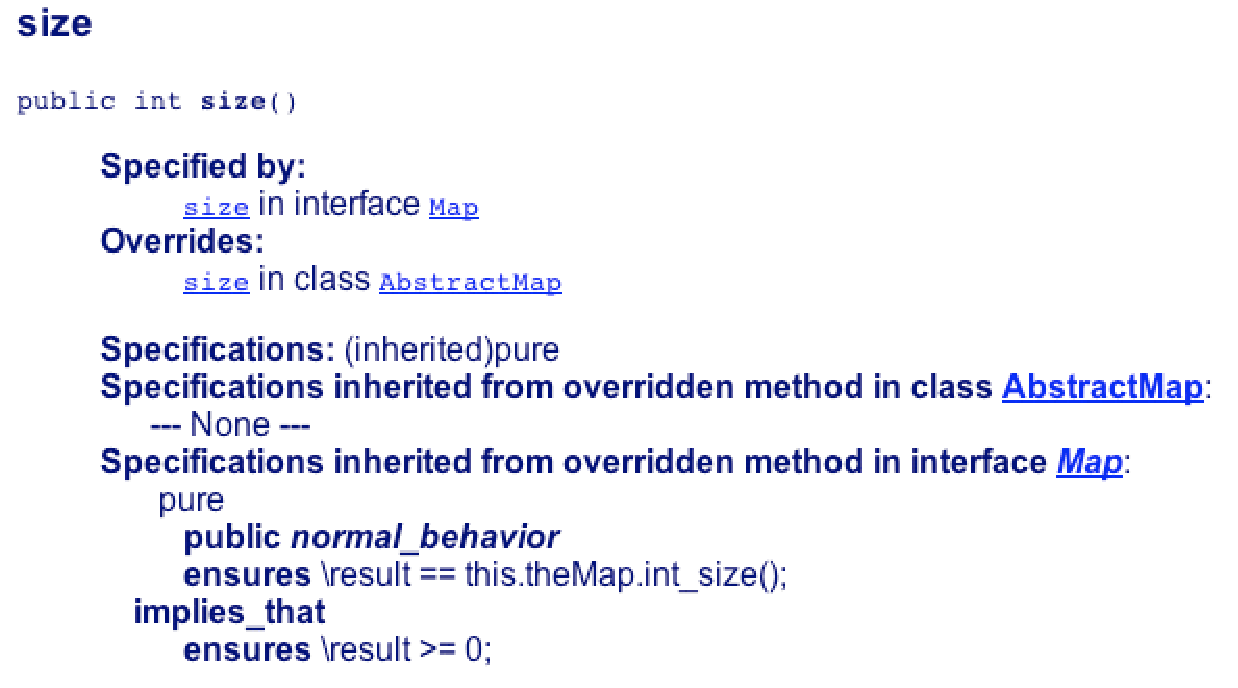
\includegraphics[width=4in]{jmldoc.pdf}
\else
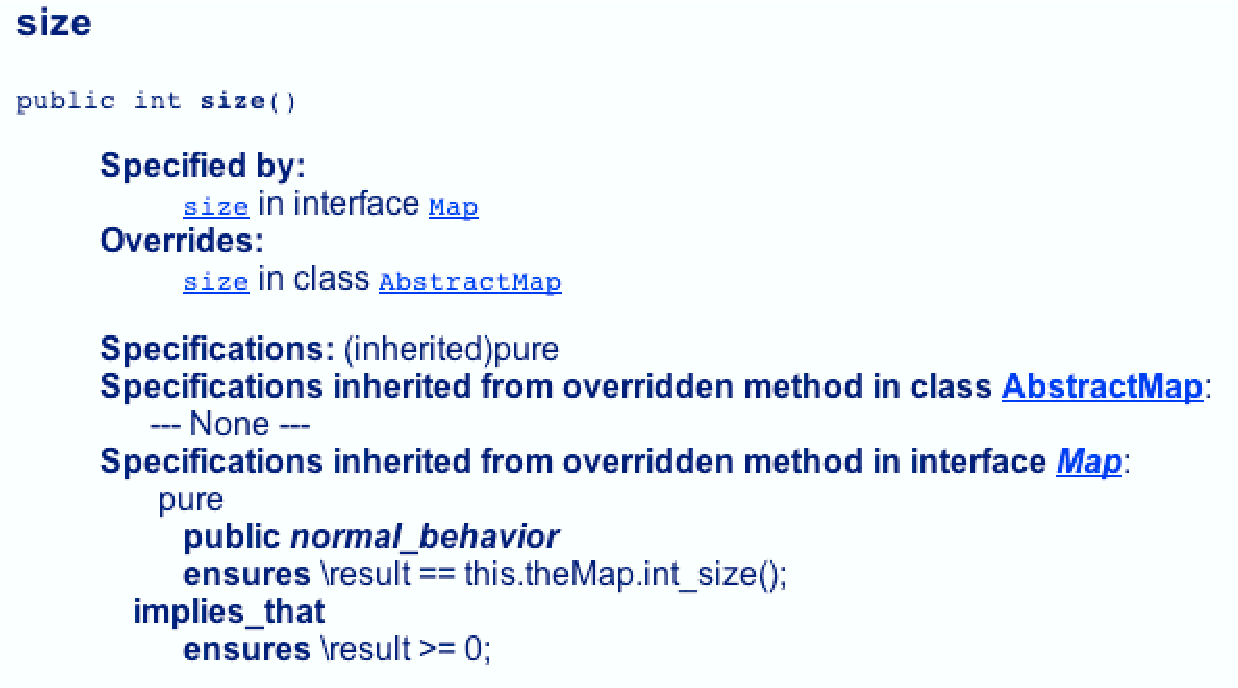
\includegraphics[width=4in]{jmldoc.eps}
\fi
% [[[Need the eps version of this.]]]
\caption{\label{jmldoc-example}Example {\JMLDOC} output}
\end{figure*}


\subsubsection{Experience}

% Experience when using the tool (describe any case studies, users...)
% - give some impression about the size of program it can handle, 
% e.g., what the biggest example that has been handled successfully
% - Some summary "Assessment of the tool".

The main experience we have with {\JMLDOC} is in documentation of
packages that ship with JML, such as JML's built-in types for modeling
and its samples, and with documentation of parts of the Java standard
libraries.  While these are used by JML users on a daily basis,
there have been no formal case studies of the usefulness of {\JMLDOC}. 
Informal reports, however, have been positive.

\subsubsection{Future Work}

% Discussion of ongoing work related to the tool's development, if any.
% Omit this subsubsection if the tool is no longer being developed.

The tool is being maintained as part of the JML toolset, but not being extended further other
than to keep pace with changes in the definition of JML itself.  Extensive maintenance is also
needed to keep pace with changes in the doclet API with each new version of Java.  As it happens,
the portions of the doclet API that are extended by {\JMLDOC} have been changing significantly
even between minor releases of {\JAVADOC}.  If this rate of change continues, the JML project may
need to seek an alternative design that is not tied as closely to the current appearance of
{\JAVADOC} documentation in order to lessen the maintenance burden. 

\subsubsection{Availability}

% Where and how to get the tool, if that's different than the JML web page.
The {\JMLDOC} tool was authored by David Cok along the lines of the goals espoused 
by Raghavan~\cite{Raghavan00}. 
It is part of the main JML toolset available via \url{www.jmlspecs.org}, 
which is developed as an open source project hosted at \url{SourceForge.net}.

%=====================================================================
\section{Applications of JML to Java Card}
\label{applications}

%% [[[Comment from referee 2:]]]
% ... the applications section is
% mainly a reference to a JavaCard study done on the basis of ESC/Java.
% This is a bit disappointing, even if several of the tool sections have
% references to user experience reports. I would suppose there would more
% documented and systematic points to make at the level of JML concerning 
% application studies overall, usability, overhead, learning curves,
% etc.
%% [[[Erik notes we should talk about the JDK specifications happening
%% at ISU.]]]

Although JML is able to specify arbitrary sequential Java programs,
most of the serious applications of JML and JML tools up to now
have targeted Java Card.  Java Card$^{TM}$ is a dialect of Java specifically
designed for the programming of the latest generation of smartcards.
Java Card is adapted to the hardware limitations of smartcards; for
instance, it does not support floating point numbers, strings, object
cloning\footnote{ The fact that Java Card does not have cloning means that 
a version of the \texttt{Purse} example in Figure~\ref{example} rewritten 
to Java Card rather than Java does verify using {\ESCJAVA}, {\LOOP}, or {\JACK}.
Indeed, the absence of \texttt{clone} in Java Card is a reason why dealing
with \texttt{clone} has not been a priority in these tools.}, 
or threads.

Java Card is a well-suited target for the application of formal
methods.  It is a relatively simple language with a restricted API\@.
Moreover, Java Card programs, called \emph{applets}, are small, typically
on the order of several KBytes of bytecode.  Additionally, correctness
of Java Card programs is of crucial importance, since they are used in
sensitive applications, e.g.\ as bank cards, identity cards, and in
mobile phones.  Furthermore, once such smartcards are issued, it is
difficult, if not impossible, to fix any software errors.

JML, and several tools for JML, have been used for Java Card,
especially in the context of the EU-supported project VerifiCard
(\url{www.verificard.org}).

JML has been used to write a formal
specification of almost the entire Java Card
API~\cite{PollBergJacobs01}.  This experience has shown that JML is
expressive enough to specify non-trivial existing API classes.  The
runtime assertion checker has been used to specify and verify a
component of a smartcard operating system~\cite{PollHarteldeJong02}.

{\ESCJAVA} has been used with great success to verify a realistic
example of an electronic purse implementation in Java
Card~\cite{CatanoHuisman02}. This case study was instrumental in
convincing industrial users of the usefulness of JML and feasibility
of automated program checking by {\ESCJAVA} for Java Card applets.
In fact, this case study
provided the motivation for the development of the  {\JACK} tool discussed
earlier, which is specifically designed for Java Card programs.  One
of the classes of the electronic purse has also been verified
using the {\LOOP} tool~\cite{BreunesseBJ02}.
An overview of the work
on this electronic purse, and the way in which {\ESCJAVA} and {\LOOP} 
can be used to complement each other,
is given in \cite{BreunesseCHJ2003}.

As witnessed by the development of the  {\JACK} tool by Gemplus, Java Card
smartcard programs may be one of the niche markets where formal
methods have a promising future. Here, the cost that companies are
willing to pay to ensure the absence of certain kinds of bugs is quite
high.  It seems that, given the current state of the art, using static
checking techniques to ensure relatively simple properties (e.g., that
no runtime exception ever reaches the top-level without being caught)
seems to provide an acceptable return-on-investment.  It should be
noted that the very simplicity of Java Card is not without its
drawbacks.  In particular, the details of its very primitive
communication with smartcards (via a byte array buffer) is not easily
abstracted away from.  It will be interesting to investigate if J2ME (Java 2
Micro Edition), which targets a wider range of electronic consumer
products, such as mobile phones and PDAs, is also an interesting
application domain for JML\@.

%=====================================================================
\section{Related Work}
\label{related}

\subsection{Java}

Many runtime assertion checkers for Java exist, for example Jass,
iContract, and Parasoft's jContract, to name just a few.  Each of
these tools has its own specification language, thus specifications
written for one tool do not work in any other tool.  And while some of
these tools support higher-level constructs such as quantifiers, all
are quite primitive when compared to JML\@.  For example, none include
support for purity specification and checking, model methods,
refinements, or unit test integration.  The developers of Jass have
expressed interest in moving to JML as their specification language.

%% We explained in Section~\ref{jmlc} why we believe that the JML
%% provides a significant advance in expressivity versus such design by
%% contract tools.

The {\CHASE} tool~\cite{CH03} is a static checker for JML's
\texttt{assignable} clauses.
It performs a syntactic check on such clauses, which, in the 
spirit of {\ESCJAVA}, is neither sound nor complete, but which spots
many mistakes made in the user's assignable clauses. 
{\CHASE} was developed to complement the functionality missing in other
tools: not checking assignable clauses was one of the sources
of unsoundness of {\ESCJAVA}. 
Also, assignable clauses are not checked by the runtime assertion 
checker, making errors in assignable clauses hard to detect.
The functionality to check assignable clauses is now incorporated 
in {\ESCJAVATWO}.
Also, the JML runtime assertion checker has started to incorporate some of this
functionality.

In addition to {\ESCJAVAS}, {\LOOP}, and {\JACK}, several other
tools exist for the verification of Java code, for instance
{\Krakatoa} \cite{MarchePaulinMohringUrbain04},
{\Jive} \cite{MeyerP00}, and
{\KeY} \cite{KeY2004}.
The {\Krakatoa} tool also uses JML as specification language;
it produces proof obligations for the theorem prover Coq.
It is planned that {\Jive} will also start supporting JML\@.
The {\KeY} tool uses OCL instead as its specification language,
and is integrated with a commercial CASE tool.

\subsection{Other languages}

SPARK (\url{www.sparkada.com}, \cite{Barnes03}) is an initiative similar to JML
in many respects, but much more mature,
and targeting Ada rather than Java.
SPARK (which stands for Spade Ada Kernel) is a language designed for 
programming high-integrity systems.  It is a subset of Ada95 
(with no object references and subclasses, for example)
enriched with annotations to enable tool support. This includes 
tools for data- and information-flow analysis, and for code verification, 
in particular to ensure the absence of runtime exceptions \cite{ChapmanAmey02}.
Spark has been successfully used to construct high-integrity systems 
that have been certified using the Common Criteria, the ISO standard for 
the certification of information technology security.
SPARK and the associated tools are marketed by Praxis Critical Systems Ltd.,
demonstrating that this technology is commercially viable.

A more recent initiative that is very similar to JML is Spec\#
\cite{BarnettLeinoSchulte04}.  The Spec\# language extends C\# with
contract specifications, analogously to the way JML extends Java.
The Spec\# compiler then introduces runtime checks for the declared 
specifications (akin to {\JMLC}), and the Boogie program verifier
tries to prove these specifications statically using an automatic
theorem prover (akin the tools described in
Section~\ref{sec:static:tools}).  One difference between Spec\# and
JML is that Spec\# builds in a new methodology for object
invariants~\cite{BarnettEtAl04a,LeinoMuller04,BarnettNaumann04},
trading restrictions on the kinds of programs that can be written for
a sound modular reasoning technique.

\subsection{OCL:  UML's constraint language}

%% [[[Comment from referee 2:]]]
% The authors clearly have major gripes against OCL. As an outsider I have
% somewhat of a difficulty understanding this. I can understand that OCL
% in general is aimed at UML, a different ballgame, true, but what are
% the conceptual difficulties in creating Java oriented instantiations
% of OCL, including a suitable semantics (which the JML tools apparently
% don't agree that much about either)? Adding a little prettyprinter would 
% probably allow such a tool to produce rather convincing JML-looking output.
% By the way I think a reference to the Key tool would be proper.

Despite the similarity in the acronyms, JML is \emph{very} different in
its aims from UML~\cite{RumbaughJacobsonBooch98}.
The most basic difference is that the UML aims to cover all phases of
analysis and design with many notations, and it tries to be independent
of programming language, while JML only deals with detailed designs
(for APIs) and is tied to Java.  The \emph{model} in
JML refers to abstract, specification-only fields that can be used to
describe the behavior of various types.  By contrast, the \emph{model} of
UML refers to the general modeling process (analysis and design) and
is not limited to abstractions of individual types.

JML does have some things in common with the Object Constraint
Language (OCL)~\cite{WarmerKleppe99}, which is part of the UML
standard.  Like JML, OCL can be used to specify invariants and pre-
and postconditions.  An important difference is that JML explicitly
targets Java, whereas OCL is not specific to any one programming
language.  One could say that JML is related to Java in the same way
that OCL is related to UML\@.

JML clearly has the disadvantage that it can not be used for, say, C++
programs, whereas OCL can.  But it also has obvious advantages when it
comes to syntax, semantics, and expressivity.  Because JML sticks to
the Java syntax and typing rules, a typical Java programmer will
prefer JML notation over OCL notation, and, for instance, prefer to
write (in JML):
\begin{verbatim}
     invariant pin != null && pin.length == 5;
\end{verbatim}
rather than the OCL:
\begin{verbatim}
     inv: pin <> null and pin->size() = 5
\end{verbatim}

JML supports all the Java modifiers such as \texttt{static},
\texttt{private}, \texttt{public}, etc., and these can be used to record
detailed design decisions for different readers.
Furthermore, there are legal Java
expressions that can be used in JML specifications but that cannot be
expressed in OCL\@.
%% [[[Like what?  Can we give an example?]]]
% Thus JML can specify more details about Java programs than would be
% possible in OCL\@.

More significant than these limitations, or differences in syntax, are
differences in semantics.  JML builds on the (well-defined) semantics
of Java. So, for instance, \texttt{equals} has the same meaning in JML
and Java, as does \texttt{==}, and the same rules for overriding,
overloading, and hiding apply.  
One cannot expect this for OCL\@,
although efforts to define a semantics for OCL are underway.
%\cite{brucker.ea:proposal:2002}.

In all, we believe that a language like JML, which is tailored to
Java, is better suited for recording the detailed design of Java
programs than a generic language like OCL\@.  Even if one uses UML in
the development of a Java application, it may be better to use JML
rather than OCL for the specification of object constraints,
especially in the later stages of the development.
There has been work on automatically translating OCL to JML \cite{Hamie04}.



% %=====================================================================
%\section{Future work}
%\label{future-work}

%% [[[Comment from referee 1:]]]
% Furthermore, the discussion about the future work that is embedded in
% the Conclusions section should be expanded, e.g., in a separate
% section, by giving a more detailed discussion or by using examples to
% illustrate the problems.  This may interest some readers who are
% considering using JML or contributing to the JML effort.

%=====================================================================
\section{Conclusions}
\label{conclusions}

We believe that JML presents a promising opportunity to gently introduce
formal specification into industrial practice. It has the following strong points:

\begin{enumerate}
\item JML is \emph{easy to learn} for any Java programmer, since its
  syntax and semantics are very close to Java.
  We believe this a crucial advantage, as a big hurdle to
  introducing formal methods in industry is often that people are not
  willing, or do not have the time, to learn yet another language.
  
\item There is no need to invest in the construction of a formal model
  before one can use JML\@. Or rather: the source code \emph{is} the
  formal model.  This brings further advantages:
  \begin{itemize}
  \item It is easy to introduce the use of JML \emph{gradually}, simply
    by adding the odd assertion to some Java code.
  \item JML can be used for existing (legacy) code and APIs.
    Indeed, most applications of JML and its tools to date
    have involved existing APIs and code.
  \item There is no discrepancy between the actual code and the formal
  model. In traditional applications of formal methods there is often a
  gap between the formal model and the actual implementation, which
  means that some bugs in the implementation cannot be found, 
  because they are not part of the formal model, and, conversely,
  some problems discovered in the formal model may not be relevant
  for the implementation.
% [[[Comment from referee 2 about the above.]]]
% The point concerning lack of discrepancies between actual code and
% formal model (p. 10): Is this really true? At the same time you're
% saying that you cannot handle lots of standard Java features (like:
% aliasing and concurrency). Also what about all the features, like
% time, memory consumption etc etc that you do not handle?

  \end{itemize}

\item There is a growing availability of a wide range of tool
      support for JML\@.
\end{enumerate}

Unlike B, JML does not impose a particular design methodology on its users.
Unlike UML, VDM, and Z, JML is tailored to specifying both the syntactic
interface of Java code and its behavior.
Therefore, JML is better suited than these alternative languages
for documenting the detailed design of existing Java programs.

\smallskip

As a common notation shared by many tools, JML offers users multiple
tools supporting the same notation.  This frees users from having to
learn a whole new language before they can start using a new tool.
The shared notation also helps the economics both for users and tool
builders.  Any industrial use of formal methods will have to be
economically justified, by comparing the costs (the extra time and
effort spent) against the benefits (improvements in quality, number of
bugs found).  Having a range of tools, offering different levels of
assurance at different costs, makes it much easier to start using JML\@.
One can begin with a technique that requires the least time and effort
(perhaps runtime assertion checking) and then move to more
labor-intensive techniques if and when that seems worthwhile, until
one has reached a combination of tools and techniques that is
cost-effective for a particular situation.

Using any of the tools for static checking or verification requires 
formal specifications of the APIs of any system libraries used, and 
the cost of developing such specifications is very high.
Indeed, the largest case study to date in using JML for specification
is the ongoing work in developing specifications for substantial parts
of the Java system libraries.
Being able to reuse these same specifications for different tools 
is an important advantage.

%% [[[From reviewer #1: The JML effort comprises tools that have been
%% specifically developed for it ( jml, jmlunit, jmldoc,...) and
%% previously existing tools that have been adapted to JML (daikon,
%% ESC/Java,...). It should be clear that for this project to work, it is
%% important to achieve a seamless integration of these tools. It may be
%% a good idea to add a few comments on the problems the authors have
%% faced to integrate these tools, and the degree of integration they
%% have achieved so far.]]]

\subsection*{Future Work}

There are still many opportunities for further development of both the
JML language and its tools. For instance, we would also like to see
support for JML in integrated development environments
(such as Eclipse) and integration with other kinds of static
checkers.  

A major recent extension to JML concerns the support for different
forms of arithmetic, providing normal mathematical integers in 
addition to Java's $n$-bit 2's-complements integers \cite{Chalin04}.

One important aspect of future work is experimenting with the
use JML for specification of real-world code and APIs, and using
the associated tools.
There has been a lot of work on producing JML specifications of the Java
system libraries (these can be downloaded from \url{www.jmlspecs.org}), 
but more work is needed.

Using JML to specify real-world code raises many interesting issues.
For instance, JML allows pure methods to be used in annotations, where 
pure methods are defined as those which have no side-effects.  
But this is a very strict definition, which can be impractical when writing
specifications, as many methods (including some in core Java libraries)
that programmers intuitively assume to be pure are not pure,
due to unobservable and benevolent side-effects \cite{Leavens-etal03b}.
Work continues on a better and more useful definition of purity,
e.g.\ \cite{BarnettEtAl04b}.

With more tools supporting JML, and the specification language
JML growing in complexity due to the different features that are
useful for the different tools, one important challenge is maintaining 
agreement on the semantics of the language between the different tools.
One thing that has become very clear in the course of developing JML 
is that precisely defining the semantics of a specification language 
such as JML is very tricky.

More generally, there are several fundamental issues in the specification 
of object-oriented systems that are still active topics of investigation.
The notion of object invariant is tricky in the presence of callbacks
\cite{BarnettEtAl04a,BarnettNaumann04,LeinoMuller04,Mueller-Poetzsch-Heffter-Leavens03a}.
Another largely open issue is how concurrency properties should be specified.

As always in imperative programming, aliasing is a major source of 
complications, and an important source of bugs.
For example, in the example in Figure~\ref{example} it is probably important
that in the constructor the field \texttt{pin} is not simply aliased
to the argument \texttt{p}, but that a new array is created.
However, the current specification does not demand this.
JML should offer practical ways to constrain potential aliasing. 
A first proposal is given in \cite{MuellerPoetzschHeffterLeavens03}.

The subtleties involved in such open problems are evidenced by the slightly
different ways in which different tools approach these problems.
This reflects the research (as opposed to industrial development)
focus of most of those involved in JML and its tools.
Nevertheless, JML seems to be successful in providing a common
notation and a semantics that is, at least for a growing core subset,
shared by many tools, and as a common notation, JML is already
proving to be useful to both tool developers and users.

\begin{acknowledgement}
Despite our long list of co-authors, still more people have been involved
in developing the tools discussed in this paper, including
Joachim van den Berg,
Abhay Bhorkar,
Kristina Boysen,
Cees-Bart Breunesse,
N\'estor Cata{\~n}o,
Patrice Chalin,
Curtis Clifton,
Kui Dai,
Werner Dietl,
Marko van Dooren,
Cormac Flanagan,
Mark Lillibridge,
Marieke Huisman,
Bart Jacobs,
Jean-Louis Lanet,
Todd Millstein,
Peter Mueller,
Greg Nelson,
Jeremy Nimmer,
Carlos Pacheco,
Arun Raghavan,
Antoine Requet,
Frederic Rioux,
Clyde Ruby,
Jim Saxe,
Raymie Stata,
Roy Tan,
and Martijn Warnier.
Thanks to Raymie Stata for his initiative in getting the JML and
{\ESCJAVA} projects to agree on a common syntax,
and to Michael M\"oller for the logo.  Work on the JML tools
at Iowa State builds on the MultiJava compiler written by Curtis
Clifton as an adaptation of the Kopi Java compiler.
\end{acknowledgement}

\bibliographystyle{plain}
\bibliography{sttt}

\end{document}

% LocalWords:  gsave moveto lineto showpage grestore INRIA Antipolis mytree
